\PassOptionsToPackage{svgnames,dvipsnames,svgnames}{xcolor}
\documentclass[acmsmall,review,anonymous,nonacm]{acmart}
\settopmatter{printfolios=true,printccs=false,printacmref=false}
%% For double-blind review submission, w/ CCS and ACM Reference
%\documentclass[acmsmall,review,anonymous]{acmart}\settopmatter{printfolios=true}
%% For single-blind review submission, w/o CCS and ACM Reference (max submission space)
%\documentclass[acmsmall,review]{acmart}\settopmatter{printfolios=true,printccs=false,printacmref=false}
%% For single-blind review submission, w/ CCS and ACM Reference
%\documentclass[acmsmall,review]{acmart}\settopmatter{printfolios=true}
%% For final camera-ready submission, w/ required CCS and ACM Reference
%\documentclass[acmsmall]{acmart}\settopmatter{}

%% Conference information
%% Supplied to authors by publisher for camera-ready submission;
%% use defaults for review submission.
\acmConference[PL'18]{ACM SIGPLAN Conference on Programming Languages}{January 01--03, 2018}{New York, NY, USA}
\acmYear{2018}
\acmISBN{} % \acmISBN{978-x-xxxx-xxxx-x/YY/MM}
\acmDOI{} % \acmDOI{10.1145/nnnnnnn.nnnnnnn}
\startPage{1}

%% Copyright information
%% Supplied to authors (based on authors' rights management selection;
%% see authors.acm.org) by publisher for camera-ready submission;
%% use 'none' for review submission.
\setcopyright{none}
%\setcopyright{acmcopyright}
%\setcopyright{acmlicensed}
%\setcopyright{rightsretained}
%\copyrightyear{2018}           %% If different from \acmYear

%% Bibliography style
% \bibliographystyle{ACM-Reference-Format}
%% Citation style
%\citestyle{acmauthoryear}  %% For author/year citations
%\citestyle{acmnumeric}     %% For numeric citations
%\setcitestyle{nosort}      %% With 'acmnumeric', to disable automatic
                            %% sorting of references within a single citation;
                            %% e.g., \cite{Smith99,Carpenter05,Baker12}
                            %% rendered as [14,5,2] rather than [2,5,14].
%\setcitesyle{nocompress}   %% With 'acmnumeric', to disable automatic
                            %% compression of sequential references within a
                            %% single citation;
                            %% e.g., \cite{Baker12,Baker14,Baker16}
                            %% rendered as [2,3,4] rather than [2-4].

%% Some recommended packages.
\usepackage{booktabs}   %% For formal tables:
                        %% http://ctan.org/pkg/booktabs
\usepackage{subcaption} %% For complex figures with subfigures/subcaptions
                        %% http://ctan.org/pkg/subcaption

%% Cyrus packages
% \usepackage{microtype}
% \usepackage{mdframed}
% \usepackage{colortab}
\usepackage{mathpartir}
% \usepackage{enumitem}
% \usepackage{bbm}
\usepackage{stmaryrd}
% \usepackage{mathtools}
% \usepackage{leftidx}
\usepackage{todonotes}
\usepackage{xspace}
% \usepackage{wrapfig}

\newcommand{\cyrus}[1]{{\color{blue} #1}}

\usepackage{listings}%
\lstloadlanguages{ML}
\lstset{tabsize=2, 
basicstyle=\footnotesize\ttfamily, 
% keywordstyle=\sffamily,
commentstyle=\itshape\ttfamily\color{gray}, 
stringstyle=\ttfamily\color{purple},
mathescape=false,escapechar=\#,
numbers=left, numberstyle=\scriptsize\color{gray}\ttfamily, language=ML, showspaces=false,showstringspaces=false,xleftmargin=15pt, 
morekeywords={string, float, int, Int, Float, String, livelit, at, SpliceRef, UpdateMonad, ViewMonad, Html, return,
capture, Typ, Exp, Option, List, Result, Dimensions, Unit},
classoffset=0,belowskip=\smallskipamount, aboveskip=\smallskipamount,
moredelim=**[is][\color{red}]{SSTR}{ESTR}
}
\newcommand{\li}[1]{\lstinline[basicstyle=\ttfamily\fontsize{9pt}{1em}\selectfont]{#1}}
\newcommand{\lismall}[1]{\lstinline[basicstyle=\ttfamily\fontsize{9pt}{1em}\selectfont]{#1}}

%% Joshua Dunfield macros
\def\OPTIONConf{1}%
\usepackage{joshuadunfield}

%% Can remove this eventually
% \usepackage{blindtext}

% \usepackage{enumitem}

%%%%%%%%%%%%%%%%%%%%%%%%%%%%%%%%%%%%%%%%%%%%%%%%%%%%%%%%%%%%%%%%%%%%%%%%%%%%%
%% Matt says: Cyrus, this package `adjustbox` seems directly related
%% to the `clipbox` error; To get rid of the error, I moved it last
%% (after other usepackages) and I added the line just above it, which
%% permits it to redefine `clipbox` (apparently also defined in
%% `pstricks`, and due to latex's complete lack of namespace
%% management, these would otherwise names clash).
% \let\clipbox\relax
% \usepackage[export]{adjustbox}% http://ctan.org/pkg/adjustbox
%%%%%%%%%%%%%%%%%%%%%%%%%%%%%%%%%%%%%%%%%%%%%%%%%%%%%%%%%%%%%%%%%%%%%%%%%%%%%%%%%


%%%%%%%%%%%%%%%%%%%%%%%%%%%%%%%%%%%%%%%%%%%%%%%%%%%%%%%%%%%%%%%%%%%%%%%%%%%%%%%%%
%\usepackage{draftwatermark}
%\SetWatermarkText{DRAFT}
%\SetWatermarkScale{1}
%%%%%%%%%%%%%%%%%%%%%%%%%%%%%%%%%%%%%%%%%%%%%%%%%%%%%%%%%%%%%%%%%%%%%%%%%%%%%%%%%


% A macro for the name of the system being described by ``this paper''
\newcommand{\HazelnutLive}{\textsf{Hazelnut Live}\xspace}
\newcommand{\Hazelnut}{\textsf{Hazelnut}\xspace}
% The mockup, work-in-progress system.
\newcommand{\Hazel}{\textsf{Hazel}\xspace}

% \newtheorem{theorem}{Theorem}[chapter]
% \newtheorem{lemma}[theorem]{Lemma}
% \newtheorem{corollary}[theorem]{Corollary}
% \newtheorem{definition}[theorem]{Definition}
% \newtheorem{assumption}[theorem]{Assumption}
% \newtheorem{condition}[theorem]{Condition}

\newtheoremstyle{slplain}% name
  {.15\baselineskip\@plus.1\baselineskip\@minus.1\baselineskip}% Space above
  {.15\baselineskip\@plus.1\baselineskip\@minus.1\baselineskip}% Space below
  {\slshape}% Body font
  {\parindent}%Indent amount (empty = no indent, \parindent = para indent)
  {\bfseries}%  Thm head font
  {.}%       Punctuation after thm head
  { }%      Space after thm head: " " = normal interword space;
        %       \newline = linebreak
  {}%       Thm head spec
\theoremstyle{slplain}
\newtheorem{thm}{Theorem}  % Numbered with the equation counter
\numberwithin{thm}{section}
\newtheorem{defn}[thm]{Definition}
\newtheorem{lem}[thm]{Lemma}
\newtheorem{prop}[thm]{Proposition}
% \newtheorem{cor}[section]{Corollary}     
% \newtheorem{lem}[section]{Lemma}         
% \newtheorem{prop}[section]{Proposition}  

% \setlength{\abovedisplayskip}{0pt}
% \setlength{\belowdisplayskip}{0pt}
% \setlength{\abovedisplayshortskip}{0pt}
% \setlength{\belowdisplayshortskip}{0pt}



\makeatletter\if@ACM@journal\makeatother
%% Journal information (used by PACMPL format)
%% Supplied to authors by publisher for camera-ready submission
\acmJournal{PACMPL}
\acmVolume{1}
\acmNumber{1}
\acmArticle{1}
\acmYear{2018}
\acmMonth{3}
\acmDOI{10.1145/nnnnnnn.nnnnnnn}
\startPage{1}
\else\makeatother
%% Conference information (used by SIGPLAN proceedings format)
%% Supplied to authors by publisher for camera-ready submission
% \acmConference[]{ACM SIGPLAN Conference on Programming Languages}{January 01--03, 2017}{New York, NY, USA}

\acmYear{2018}
\acmISBN{978-x-xxxx-xxxx-x/YY/MM}
\acmDOI{10.1145/nnnnnnn.nnnnnnn}
\startPage{1}
\fi


%% Copyright information
%% Supplied to authors (based on authors' rights management selection;
%% see authors.acm.org) by publisher for camera-ready submission
\setcopyright{none}             %% For review submission
%\setcopyright{acmcopyright}
%\setcopyright{acmlicensed}
%\setcopyright{rightsretained}
%\copyrightyear{2017}           %% If different from \acmYear


\fancyfoot{} % suppresses the footer (also need \thispagestyle{empty} after \maketitle below)


%% Bibliography style
\bibliographystyle{ACM-Reference-Format}
%% Citation style
%% Note: author/year citations are required for papers published as an
%% issue of PACMPL.
% \citestyle{acmauthoryear}   %% For author/year citations

% !TEX root = main.tex

\newcommand{\mynote}[3]{\textcolor{#3}{\textsf{{#2}}}}
\newcommand{\rkc}[1]{\mynote{rkc}{#1}{blue}}
\newcommand{\cy}[1]{\mynote{cy}{#1}{purple}}
\newcommand{\mah}[1]{\mynote{cy}{#1}{green}}
\newcommand{\matt}[1]{{\color{blue}{\textit{Matt:~#1}}}}

\newcommand{\cvert}{{\,{\vert}\,}}

%% https://tex.stackexchange.com/questions/9796/how-to-add-todo-notes
\newcommand{\rkcTodo}[1]{\todo[linecolor=blue,backgroundcolor=blue!25,bordercolor=blue]{#1}}

\newcommand{\mattTodo}[1]{\todo[linecolor=green,backgroundcolor=green!2,bordercolor=green]{\tiny\textit{#1}}}
\newcommand{\mattOmit}[1]{\colorbox{yellow}{(Matt omitted stuff here)}}

% \usepackage{amssymb}% http://ctan.org/pkg/amssymb
\usepackage{pifont}% http://ctan.org/pkg/pifont
\newcommand{\cmark}{\ding{51}}%
\newcommand{\xmark}{\ding{55}}%

\def\parahead#1{\paragraph{\textbf{#1.}}}
%% \def\paraheadNoDot#1{\paragraph{{\textbf{#1}}}}
\def\subparahead#1{\paragraph{\textit{#1.}}}
%% \def\paraheadindent#1{\paragraph{}\textit{#1.}}
%% \def\paraheadindentnodot#1{\paragraph{}\textit{#1}}

% \newcommand{\ie}{{\emph{i.e.}}}
% \newcommand{\eg}{{\emph{e.g.}}}
% \newcommand{\etc}{{\emph{etc.}}}
% \newcommand{\cf}{{\emph{cf.}}}
% \newcommand{\etal}{{\emph{et al.}}}

%% \newcommand{\hazel}{\ensuremath{\textsc{Hazel}}}
%% \newcommand{\sns}{\ensuremath{\textsc{Sketch-n-Sketch}}}
%% \newcommand{\deuce}{\ensuremath{\textsc{Deuce}}}
\newcommand{\Elm}{\ensuremath{\textsf{Elm}}}
\newcommand{\sns}
  %% {\ensuremath{\textrm{Sketch-n-Sketch}}}
  {\ensuremath{\textsf{Sketch-n-Sketch}}}
\newcommand{\deuce}
  %% {\ensuremath{\textrm{Deuce}}}
  {\ensuremath{\textsf{Deuce}}}

\newcommand{\sectionDescription}[1]{\section{#1}}
\newcommand{\subsectionDescription}[1]{\subsection{#1}}
\newcommand{\subsubsectionDescription}[1]{\subsubsection{#1}}
%% \newcommand{\subsectionDescription}[1]{\subsection*{#1}}
\newcommand{\suppMaterials}{the Supplementary Materials}

\newcommand{\defeq}{\overset{\textrm{def}}{=}}

\newcommand{\eap}{action suggestion panel\xspace}
\newcommand{\Eap}{Action suggestion panel\xspace}

\newcommand{\myfootnote}[1]{\footnote{ #1}}

\def\sectionautorefname{Section}
\def\subsectionautorefname{Section}
\def\subsubsectionautorefname{Section}

\newcommand{\code}[1]{\lstinline{#1}}

% Make italic?
%\newcommand{\Property}[1]{\emph{#1}}
\newcommand{\Property}[1]{\textrm{#1}}

% Calling out Cyrus's favorite verb, 'to be' ;)
\newcommand{\IS}{\colorbox{red}{is}\xspace}

\newcommand{\codeSize}
  %% {\footnotesize}
  {\small}

%\newcommand{\JoinTypes}[2]{\textsf{join}~~#1~~#2}
\newcommand{\JoinTypes}[2]{\textsf{join}(#1,#2)}

%%%%%%%%%%%%%%%%%%%%%%%%%%%%%%%%%%%%%%%%%%%%%%%%%%%%%%%%%%%%%%%%%%%%%%%%%%%%%%%%
%% Spacing

\newcommand{\sep}{\hspace{0.06in}}
\newcommand{\sepPremise}{\hspace{0.20in}}
\newcommand{\hsepRule}{\hspace{0.20in}}
\newcommand{\vsepRuleHeight}{0.08in}
\newcommand{\vsepRule}{\vspace{\vsepRuleHeight}}
\newcommand{\miniSepOne}{\hspace{0.01in}}
\newcommand{\miniSepTwo}{\hspace{0.02in}}
\newcommand{\miniSepThree}{\hspace{0.03in}}
\newcommand{\miniSepFour}{\hspace{0.04in}}
\newcommand{\miniSepFive}{\hspace{0.05in}}

%%%%%%%%%%%%%%%%%%%%%%%%%%%%%%%%%%%%%%%%%%%%%%%%%%%%%%%%%%%%%%%%%%%%%%%%%%%%%%%%

% \lstset{
% %mathescape=true,basicstyle=\fontsize{8}{9}\ttfamily,
% literate={=>}{$\Rightarrow$}2
%          {<=}{$\leq$}2
%          {->}{${\rightarrow}$}1
%          {\\\\=}{\color{red}{$\lambda$}}2
%          {\\\\}{$\lambda$}2
%          {**}{$\times$}2
%          {*.}{${\color{blue}{\texttt{*.}}}$}2
%          {+.}{${\color{blue}{\texttt{+.}}}$}2
%          {<}{${\color{green}{\lhd}}$}1
%          {>?}{${\color{green}{\rhd}}$?}2
%          {<<}{${\color{green}{\blacktriangleleft}}$}1
%          {>>?}{${\color{green}{\blacktriangleright}}$?}2
%          {\{}{${\color{blue}{\{}}$}1
%          {\}}{${\color{blue}{\}}}$}1
%          {[}{${\color{purple}{[}}$}1
%          {]}{${\color{purple}{]}}$}1
%          {(}{${\color{darkgray}{\texttt{(}}}$}1
%          {)}{${\color{darkgray}{\texttt{)}}}$}1
%          {]]}{${\color{gray}{\big(}}$}1
%          {]]}{${\color{gray}{\big)}}$}1
% }

% !TEX root = hazelnut-dynamics.tex

% \newcommand{\Label}[1]{\vspace{-20px}\label{#1}%
%   {\small\textcolor{cyan}{(\texttt{#1})}}\vspace{20px}%
% }

\newcommand{\cmttclo}[2]{\mathsf{clo}(#1, #2)}

% \newcommand{\CaptionLabel}[2]{
%   \caption{#1 {\small\textcolor{cyan}{(#2)}}}
%   \label{#2}}
\newcommand{\CaptionLabel}[2]{
  \caption{#1}
  \label{#2}}

% Violet hotdogs; highlight color helps distinguish them
\newcommand{\llparenthesiscolor}{\textcolor{violet}{\llparenthesis}}
\newcommand{\rrparenthesiscolor}{\textcolor{violet}{\rrparenthesis}}
% \newcommand{\llparenthesiscolor}{\textcolor{red}{\lfloor}}
% \newcommand{\rrparenthesiscolor}{\textcolor{red}{\rfloor}}

%% TODO if feeling really obsessive, use the following in place of x,u,c,b
\newcommand{\varVar}{x}
\newcommand{\varHole}{u}
\newcommand{\econst}{c}
\newcommand{\tbase}{b}

% HTyp and HExp
\newcommand{\isComplete}[1]{#1~\mathsf{complete}}

% HTyp
\newcommand{\tarr}[2]{#1 \rightarrow #2}
%\newcommand{\tsum}[2]{#1 + #2}
\newcommand{\tprod}[2]{#1 \times #2}
\newcommand{\tnum}{\texttt{num}}
\newcommand{\tb}{\texttt{b}}
\newcommand{\tehole}{\llparenthesiscolor\rrparenthesiscolor}
\newcommand{\tsum}[2]{{#1} + {#2}}

\newcommand{\tconsistent}[2]{#1 \sim #2}
\newcommand{\tinconsistent}[2]{#1 \nsim #2}

% HExp
\newcommand{\hlam}[2]{\lambda #1.#2}
\newcommand{\halam}[3]{\lambda #1{:}#2.#3}
\newcommand{\hap}[2]{#1(#2)}
\newcommand{\hapP}[2]{(#1)~(#2)} % Extra paren around function term
\newcommand{\hpair}[2]{(#1, #2)}
\newcommand{\hprj}[2]{\mathsf{prj}_{#1}(#2)}
\newcommand{\lblL}{\mathsf{L}}
\newcommand{\lblR}{\mathsf{R}}
\newcommand{\hnum}[1]{\underline{#1}}
%\newcommand{\hcase}[5]{\mathsf{case}\,#1\,\mathsf{of}\,#2\Rightarrow#3~\vert~#4\Rightarrow#5}
\newcommand{\hadd}[2]{#1 + #2}
\newcommand{\hehole}[1]{\llparenthesiscolor\rrparenthesiscolor^{#1}}
% \newcommand{\hhole}[1]{\setlength{\fboxsep}{0pt}\fcolorbox{red}{white}{\vphantom{)}$#1$}}
\newcommand{\hhole}[2]{\llparenthesiscolor#1\rrparenthesiscolor^{#2}}
% \newcommand{\hhole}[1]{
  % \setlength{\fboxsep}{0pt}
  % \colorbox{violet!10!white!100}{\ensuremath{\llparenthesiscolor#1\rrparenthesiscolor}}}
\newcommand{\hindet}[1]{\lceil#1\rceil}
%\newcommand{\hinj}[2]{\texttt{inj}_{#1}({#2})}
\newcommand{\hinL}[1]{\mathsf{inl}(#1)}
\newcommand{\hinR}[1]{\mathsf{inr}(#1)}
\newcommand{\hcase}[5]{\texttt{case}({#1},{#2}.{#3},{#4}.{#5})}

\newcommand{\hGamma}{\Gamma}
\newcommand{\EmptyhGamma}{\emptyset} % From hand-written notes, Canonical forms lemma; page 14
\newcommand{\EmptyDelta}{\cdot} % From hand-written notes, ES-Const rule, page 1
\newcommand{\domof}[1]{\text{dom}(#1)}
\newcommand{\hsyn}[3]{#1 \vdash #2 \Rightarrow #3}
\newcommand{\hana}[3]{#1 \vdash #2 \Leftarrow #3}

% ZTyp and ZExp
\newcommand{\zlsel}[1]{{\bowtie}{#1}}
\newcommand{\zrsel}[1]{{#1}{\bowtie}}

%\newcommand{\zwsel}[1]{\adjustbox{cframe=blue}{\ensuremath{{\textcolor{blue}{\triangleright}}{#1}{\textcolor{blue}{\triangleleft}}}}}
\newcommand{\zwsel}[1]{
  \setlength{\fboxsep}{0pt}
  \colorbox{green!10!white!100}{
    \ensuremath{{{\textcolor{Green}{{\hspace{-2px}\triangleright}}}}{#1}{\textcolor{Green}{\triangleleft{\vphantom{\tehole}}}}}}
}
%\newcommand{\zwsel}[1]{{\triangleright}{#1}{\triangleleft}}

\newcommand{\removeSel}[1]{#1^{\diamond}}

% ZTyp
\newcommand{\ztau}{\hat{\tau}}

% ZExp
\newcommand{\zexp}{\hat{e}}

% Direction
\newcommand{\dParent}{\mathtt{parent}}
\newcommand{\dChild}{\mathtt{firstChild}}
\newcommand{\dNext}{\mathtt{nextSib}}
\newcommand{\dPrev}{\mathtt{prevSib}}

% Action
\newcommand{\aMove}[1]{\mathtt{move}~#1}
	\newcommand{\zrightmost}[1]{\mathsf{rightmost}(#1)}
	\newcommand{\zleftmost}[1]{\mathsf{leftmost}(#1)}
\newcommand{\aSelect}[1]{\mathtt{sel}~#1}
\newcommand{\aDel}{\mathtt{del}}
\newcommand{\aReplace}[1]{\mathtt{replace}~#1}
\newcommand{\aConstruct}[1]{\mathtt{construct}~#1}
\newcommand{\aConstructx}[1]{#1}
\newcommand{\aFinish}{\mathtt{finish}}

\newcommand{\performAna}[5]{#1 \vdash #2 \xlongrightarrow{#4} #5 \Leftarrow #3}
\newcommand{\performAnaI}[5]{#1 \vdash #2 \xlongrightarrow{#4}\hspace{-3px}{}^{*}~ #5 \Leftarrow #3}
\newcommand{\performSyn}[6]{#1 \vdash #2 \Rightarrow #3 \xlongrightarrow{#4} #5 \Rightarrow #6}
\newcommand{\performSynI}[6]{#1 \vdash #2 \Rightarrow #3 \xlongrightarrow{#4}\hspace{-3px}{}^{*}~ #5 \Rightarrow #6}
\newcommand{\performTyp}[3]{#1 \xlongrightarrow{#2} #3}
\newcommand{\performTypI}[3]{#1 \xlongrightarrow{#2}\hspace{-3px}{}^{*}~#3}

\newcommand{\performMove}[3]{#1 \xlongrightarrow{#2} #3}
\newcommand{\performDel}[2]{#1 \xlongrightarrow{\aDel} #2}

% Form
\newcommand{\farr}{\mathtt{arrow}}
\newcommand{\fnum}{\mathtt{num}}
\newcommand{\fsum}{\mathtt{sum}}

\newcommand{\fasc}{\mathtt{asc}}
\newcommand{\fvar}[1]{\mathtt{var}~#1}
\newcommand{\flam}[1]{\mathtt{lam}~#1}
\newcommand{\fap}{\mathtt{ap}}
\newcommand{\farg}{\mathtt{arg}}
\newcommand{\fnumlit}[1]{\mathtt{lit}~#1}
\newcommand{\fplus}{\mathtt{plus}}
\newcommand{\fhole}{\mathtt{hole}}
\newcommand{\fnehole}{\mathtt{nehole}}

\newcommand{\finj}[1]{\mathtt{inj}~#1}
\newcommand{\fcase}[2]{\mathtt{case}~#1~#2}

% Talk about formal rules in example
\newcommand{\refrule}[1]{\textrm{Rule~(#1)}}

\newcommand{\herase}[1]{\left|#1\right|_\textsf{erase}}

\newcommand{\arrmatch}[2]{#1 \blacktriangleright_{\rightarrow} #2}
%% TODO maybe write underbracket
%% \newcommand{\groundmatch}[2]{\underline{#1} = #2}
\newcommand{\groundmatch}[2]{#1 \blacktriangleright_{\mathsf{ground}} #2}
\newcommand{\prodmatch}[2]{#1 \blacktriangleright_{\times} #2}
\newcommand{\summatch}[2]{#1 \blacktriangleright_{+} #2}


\newcommand{\TABperformAna}[5]{#1 \vdash & #2                & \xlongrightarrow{#4} & #5 & \Leftarrow #3}
\newcommand{\TABperformSyn}[6]{#1 \vdash & #2 \Rightarrow #3 & \xlongrightarrow{#4} & #5 \Rightarrow #6}
\newcommand{\TABperformTyp}[3]{& #1 & \xlongrightarrow{#2} & #3}

\newcommand{\TABperformMove}[3]{#1 & \xlongrightarrow{#2} & #3}
\newcommand{\TABperformDel}[2]{#1 \xlongrightarrow{\aDel} #2}

\newcommand{\sumhasmatched}[2]{#1 \mathrel{\textcolor{black}{\blacktriangleright_{+}}} #2}

%%%% DYNAMICS %%%%
%% TODO remove these macros
%% marks for eval
\newcommand{\unevaled}{\times}
\newcommand{\evaled}{\checkmark}
\newcommand{\markname}{m}

\newcommand{\mvar}[0]{u}
\newcommand{\subst}[0]{\sigma}
\newcommand{\substitute}[3]{[#1/#2]#3}
\newcommand{\fvof}[1]{\mathsf{FV}(#1)}
\newcommand{\dexp}[0]{d}
\newcommand{\dconst}[0]{c}
\newcommand{\dval}[0]{\ddot{v}}
%% TODO remove this macro
\newcommand{\dcast}[2]{\langle #1 \rangle ~ #2}
%% TODO make the following two look better
\newcommand{\dcasttwo}[3]{#1 \langle{#2}\Rightarrow{#3}\rangle}
\newcommand{\dcastthree}[4]
  {#1 \langle{#2}\Rightarrow{#3}\Rightarrow{#4}\rangle} %% sugared version
  %% {\dcasttwo{\dcasttwo{#1}{#2}{#3}}{#3}{#4}} %% unsugared version
\newcommand{\dcastfail}[3]{#1 \langle{#2}\Rightarrow{\tehole}\not\Rightarrow{#3}\rangle}
%% \newcommand{\dlam}[3]{\lambda #1:#2.#3}
\newcommand{\dlam}[3]{\halam{#1}{#2}{#3}}
\newcommand{\dap}[2]{#1(#2)}
\newcommand{\dapP}[2]{(#1)(#2)} % Extra paren around function term
\newcommand{\dnum}[1]{\underline{#1}}
%\newcommand{\dcase}[5]{\mathsf{case}\,#1\,\mathsf{of}\,#2\Rightarrow#3~\vert~#4\Rightarrow#5}
\newcommand{\dadd}[2]{#1 + #2}
%% TODO third arg should be empty
\newcommand{\dehole}[3]{\leftidx{^{#3}}{\llparenthesiscolor\rrparenthesiscolor}{^{#1}_{#2}}}
%% TODO fourth arg should be empty
\newcommand{\dhole}[4]{\leftidx{^{#4}}{\llparenthesiscolor#1\rrparenthesiscolor}{^{#2}_{#3}}}
\newcommand{\dindet}[1]{\lceil#1\rceil}
%\newcommand{\dinj}[2]{\texttt{inj}_{#1}({#2})}
\newcommand{\dinL}[2]{\mathsf{inl}_{#1}(#2)}
\newcommand{\dinR}[2]{\mathsf{inr}_{#1}(#2)}
\newcommand{\dcase}[5]{\texttt{case}({#1},{#2}.{#3},{#4}.{#5})}
\newcommand{\dpair}[2]{(#1,#2)}
\newcommand{\dprj}[2]{\mathsf{prj}_{#1}(#2)}

\newcommand{\expandAna}[6]{#1 \vdash #2 \Leftarrow #3 \leadsto #4 : #5 \dashv #6}
\newcommand{\expandSyn}[5]{#1 \vdash #2 \Rightarrow #3 \leadsto #4 \dashv #5}
\newcommand{\hasType}[4]{#1; #2 \vdash #3 : #4}
\newcommand{\isValue}[1]{#1~\mathsf{val}}
\newcommand{\isGround}[1]{#1~\mathsf{ground}}
\newcommand{\isBoxedValue}[1]{#1~\mathsf{boxedval}}
\newcommand{\isIndet}[1]{#1~\mathsf{indet}}
\newcommand{\isFinal}[1]{#1~\mathsf{final}}
\newcommand{\isErr}[2]{#1 \vdash #2~\mathsf{err}}
%% \newcommand{\stepsTo}[2]{#1 \mapsto_{\Delta} #2}
%% TODO first arg should be empty
%% \newcommand{\stepsToD}[3]{#1 \vdash #2 \mapsto #3}
\newcommand{\stepsToD}[3]{#2 \mapsto #3}
\newcommand{\multiStepsTo}[2]{#1 \mapsto^* #2}

%% TODO if feeling obsessive, replace direct uses of \Delta
\newcommand{\hDelta}{\Delta}
\newcommand{\Dunion}[2]{#1 \cup #2}
\newcommand{\idof}[1]{\mathsf{id}(#1)}
\newcommand{\Dbinding}[3]{#1 :: #3[#2]}
\newcommand{\instantiate}[3]{\llbracket#1 / #2\rrbracket #3}

% Contextual dynamics
\newcommand{\evalctx}{\mathcal{E}}
\newcommand{\evalhole}{\circ}
\newcommand{\isevalctx}[1]{#1~\mathsf{evalCtx}}
%% TODO first arg should be empty
%% \newcommand{\reducesE}[3]{#1 \vdash #2 \longrightarrow #3}
\newcommand{\reducesE}[3]{#2 \longrightarrow #3}
\newcommand{\selectEvalCtxR}[2]{#1\{#2\}}
\newcommand{\selectEvalCtx}[3]{#1=\selectEvalCtxR{#2}{#3}}
\newcommand{\maybePremise}[1]{{\textcolor{red}[}#1{\textcolor{red}]}}

\newcommand{\inhole}[2]{\mathsf{inhole}(#1; #2)}

\newcommand{\DoSubst}[3]{[#1/#2]{#3}}


\setlength{\abovecaptionskip}{4pt plus 3pt minus 2pt} % Chosen fairly arbitrarily
\setlength{\belowcaptionskip}{-4pt plus 3pt minus 2pt} % Chosen fairly arbitrarily


\begin{document}

%% Title information
\title
  [Filling Typed Holes with Live GUIs]
  {Filling Typed Holes with Live GUIs}
  %% [Programming by Direct Manipulation of Palettes]
  %% {Functional Programming by\\Direct Manipulation of Live Palette Expressions}

                                        %% when present, will be used in
                                        %% header instead of Full Title.
% \titlenote{with title note}             %% \titlenote is optional;
                                        %% can be repeated if necessary;
                                        %% contents suppressed with 'anonymous'
% \subtitle{Subtitle}                     %% \subtitle is optional
% \subtitlenote{with subtitle note}       %% \subtitlenote is optional;
                                        %% can be repeated if necessary;
                                        %% contents suppressed with 'anonymous'


%% Author information
%% Contents and number of authors suppressed with 'anonymous'.
%% Each author should be introduced by \author, followed by
%% \authornote (optional), \orcid (optional), \affiliation, and
%% \email.
%% An author may have multiple affiliations and/or emails; repeat the
%% appropriate command.
%% Many elements are not rendered, but should be provided for metadata
%% extraction tools.

%% Author with single affiliation.
\author{Cyrus Omar}
% \authornote{with author1 note}          %% \authornote is optional;
                                        %% can be repeated if necessary
% \orcid{nnnn-nnnn-nnnn-nnnn}             %% \orcid is optional
\affiliation{
  % \position{Position1}
  % \department{Department1}              %% \department is recommended
  \institution{University of Michigan}            %% \institution is required
  % \streetaddress{Street1 Address1}
  % \city{City1}
  % \state{State1}
  % \postcode{Post-Code1}
  % \country{Country1}
}
\email{comar@cs.uchicago.edu}          %% \email is recommended

\author{Nick Collins}
% \authornote{with author1 note}          %% \authornote is optional;
                                        %% can be repeated if necessary
% \orcid{nnnn-nnnn-nnnn-nnnn}             %% \orcid is optional
\affiliation{
  % \position{Position1}
  % \department{Department1}              %% \department is recommended
  \institution{University of Chicago}            %% \institution is required
  % \streetaddress{Street1 Address1}
  % \city{City1}
  % \state{State1}
  % \postcode{Post-Code1}
  % \country{Country1}
}
\email{nickmc@uchicago.edu}          %% \email is recommended

\author{David Moon}
% \authornote{with author1 note}          %% \authornote is optional;
                                        %% can be repeated if necessary
% \orcid{nnnn-nnnn-nnnn-nnnn}             %% \orcid is optional
\affiliation{
  % \position{Position1}
  % \department{Department1}              %% \department is recommended
  \institution{University of Michigan}            %% \institution is required
  % \streetaddress{Street1 Address1}
  % \city{City1}
  % \state{State1}
  % \postcode{Post-Code1}
  % \country{Country1}
}
\email{dmoo@umich.edu}          %% \email is recommended


\author{Ian Voysey}
% \authornote{with author1 note}          %% \authornote is optional;
                                        %% can be repeated if necessary
% \orcid{nnnn-nnnn-nnnn-nnnn}             %% \orcid is optional
\affiliation{
  % \position{Position1}
  % \department{Department1}              %% \department is recommended
  \institution{Carnegie Mellon University}            %% \institution is required
  % \streetaddress{Street1 Address1}
  % \city{City1}
  % \state{State1}
  % \postcode{Post-Code1}
  % \country{Country1}
}
\email{iev@cs.cmu.edu}          %% \email is recommended

\author{Ravi Chugh}
% \authornote{with author1 note}          %% \authornote is optional;
                                        %% can be repeated if necessary
% \orcid{nnnn-nnnn-nnnn-nnnn}             %% \orcid is optional
\affiliation{
  % \position{Position1}
  % \department{Department1}              %% \department is recommended
  \institution{University of Chicago}            %% \institution is required
  % \streetaddress{Street1 Address1}
  % \city{City1}
  % \state{State1}
  % \postcode{Post-Code1}
  % \country{Country1}
}
\email{rchugh@cs.uchicago.edu}          %% \email is recommended

\author{Ravi Chugh}
% \authornote{with author1 note}          %% \authornote is optional;
                                        %% can be repeated if necessary
% \orcid{nnnn-nnnn-nnnn-nnnn}             %% \orcid is optional
\affiliation{
  % \position{Position1}
  % \department{Department1}              %% \department is recommended
  \institution{University of Chicago}            %% \institution is required
  % \streetaddress{Street1 Address1}
  % \city{City1}
  % \state{State1}
  % \postcode{Post-Code1}
  % \country{Country1}
}
\email{rchugh@cs.uchicago.edu}          %% \email is recommended

% %% Author with two affiliations and emails.
% \author{First2 Last2}
% \authornote{with author2 note}          %% \authornote is optional;
%                                         %% can be repeated if necessary
% \orcid{nnnn-nnnn-nnnn-nnnn}             %% \orcid is optional
% \affiliation{
%   \position{Position2a}
%   \department{Department2a}             %% \department is recommended
%   \institution{Institution2a}           %% \institution is required
%   \streetaddress{Street2a Address2a}
%   \city{City2a}
%   \state{State2a}
%   \postcode{Post-Code2a}
%   \country{Country2a}
% }
% \email{first2.last2@inst2a.com}         %% \email is recommended
% \affiliation{
%   \position{Position2b}
%   \department{Department2b}             %% \department is recommended
%   \institution{Institution2b}           %% \institution is required
%   \streetaddress{Street3b Address2b}
%   \city{City2b}
%   \state{State2b}
%   \postcode{Post-Code2b}
%   \country{Country2b}
% }
% \email{first2.last2@inst2b.org}         %% \email is recommended


%% Paper note
%% The \thanks command may be used to create a "paper note" ---
%% similar to a title note or an author note, but not explicitly
%% associated with a particular element.  It will appear immediately
%% above the permission/copyright statement.
% \thanks{with paper note}                %% \thanks is optional
                                        %% can be repeated if necesary
                                        %% contents suppressed with 'anonymous'


%% Abstract
%% Note: \begin{abstract}...\end{abstract} environment must come
%% before \maketitle command
% !TEX root = palettes-paper.tex

\begin{abstract}

Palettes... \cite{popl-paper}

\end{abstract}



%% 2012 ACM Computing Classification System (CSS) concepts
%% Generate at 'http://dl.acm.org/ccs/ccs.cfm'.
% \begin{CCSXML}
% <ccs2012>
% <concept>
% <concept_id>10011007.10011006.10011008</concept_id>
% <concept_desc>Software and its engineering~General programming languages</concept_desc>
% <concept_significance>500</concept_significance>
% </concept>
% <concept>
% <concept_id>10003456.10003457.10003521.10003525</concept_id>
% <concept_desc>Social and professional topics~History of programming languages</concept_desc>
% <concept_significance>300</concept_significance>
% </concept>
% </ccs2012>
% \end{CCSXML}

% \ccsdesc[500]{Software and its engineering~General programming languages}
% \ccsdesc[300]{Social and professional topics~History of programming languages}
%% End of generated code


%% Keywords
%% comma separated list
% \keywords{keyword1, keyword2, keyword3}  %% \keywords is optional
% \keywords{Live Programming, Palettes, Hazel, Code Editors}


%% \maketitle
%% Note: \maketitle command must come after title commands, author
%% commands, abstract environment, Computing Classification System
%% environment and commands, and keywords command.
\maketitle
% \thispagestyle{empty} % suppresses the footer

% \section{TODO List}

% \begin{itemize}

% \item[\cmark] palette macros
% \item action semantics
% \item \Hazel{} in \Hazel{} (sums, productions, recursive types)
% \item palette functions
% \item live palettes
% \item synthetic (or fancy record-type-level-computation) (or not-fancy untyped) palettes
% \item parameterized palettes
% \item palette-specific actions
% \item option to render palette macro expansion as expression or value
% \item \Hazel{} UI: ``formula bar'' for expressions
% \item \sns{} implementation
% \item examples!

% \end{itemize}

\section{Introduction}\label{sec:intro}
Text-based program editors are flexible and expressive user interfaces
so it is little wonder that they remain dominant decades after the teletype.
However, textual user interfaces are not the best tool for every computational job.
% In particular, there are countless 
% data types for which a non-textual
% user interface may situationally be more appropriate.

As a simple example, consider a record type
classifying RGBA-encoded colors. 
It is possible to select a particular color by entering
an expression of this type in a text editor, e.g. \li{\{ r: 255, g: 178, b: 45, a: 100 \}}. 
The problem with this textual user interface for color selection is that 
it offers no live feedback about which color has been selected 
and limited editing affordances for tweaking the selected color.
Analagous critiques apply to strictly textual user interfaces for 
countless other data structures,
such as vector graphics,
animation parameters,
musical sequences,
audio filters,
board game states, 
GUI widgets and layouts,
tabular data, 
plots,
geospatial data, 
neural network diagrams, 
biological neuron models, 
mathematical diagrams, 
and so on.

% It is difficult for the programmer, or anyone subsequently reading or modifying the code, to know which color is represented
% and to interactively tweak that color.

Practitioners in domains where manipulating data of types like these is 
a central activity 
have largely eschewed general-purpose programming environments 
in favor of more specialized graphical end-user applications, like %
image and video editors, music composition software, level design tools, 
and bespoke GUIs written by students or lab technicians, 
in large part because these applications 
take seriously the need for domain-specific forms of live feedback, 
graphical data representations, and 
direct manipulation affordances, 
e.g. color palettes, visual timelines, interactive plots, and maps.

The tragedy is that these applications have 
limited support for abstraction and composition.
It is difficult, for example, to bind a
color to a variable for use in multiple locations in an
otherwise directly constructed game map,
or to define a function that computes portions of an 
otherwise directly constructed vector graphic,
or to transform a directly constructed musical sequence 
by passing it through a series of symbolically defined functions.
Moreover, it is difficult to add new affordances or to compose
affordances in ways that the application developer did not anticipate.
Users cannot easily make even simple changes like replacing a numeric text box in a dialog with a slider,
much less more ambitious changes like installing an alternative visual interface for expressing geospatial data queries 
into a database frontend.

% Better support for manipulating data of types like these would be particularly helpful for users engaging in
% live and exploratory programming in domains like web design, media production,
% and data analysis. Indeed, 

This paper aims to resolve this tension between
programmatic and direct manipulation user interfaces by designing 
a programming environment that
is able to surface GUIs when working with types for which
they are useful, while retaining full support for symbolic program manipulation
and the abstraction and composition mechanisms
available in modern general-purpose programming languages.

\subsection{Background}\label{sec:background}
\definecolor{mygray}{rgb}{0.93, 0.93, 0.93}
\definecolor{shadecolor}{named}{mygray}

\begin{figure*}
  \begin{minipage}[t]{0.37\textwidth}
    \begin{subfigure}[t]{\linewidth}
    \begin{snugshade}
      \vspace*{-2mm}
      \caption{\textbf{Prior Work:} Graphite \cite{Graphite}}
       \label{fig:graphite}
      \vspace*{1mm}
     \end{snugshade}
      \vspace*{-1mm}
      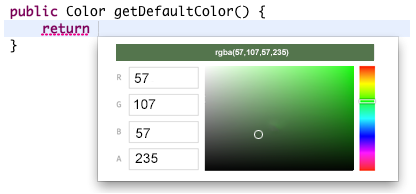
\includegraphics[width=\linewidth]{graphite-color-palette-green.png}
      \vspace*{-5mm}
    \end{subfigure}
    \hspace{8mm}
    \begin{subfigure}[t]{\linewidth}
     \begin{snugshade}
      \vspace*{-2mm}
      \caption{\textbf{This Paper:} Livelits are live and compositional}
    \label{fig:color}
      \vspace*{1mm}
     \end{snugshade}
      \vspace*{-1mm}
      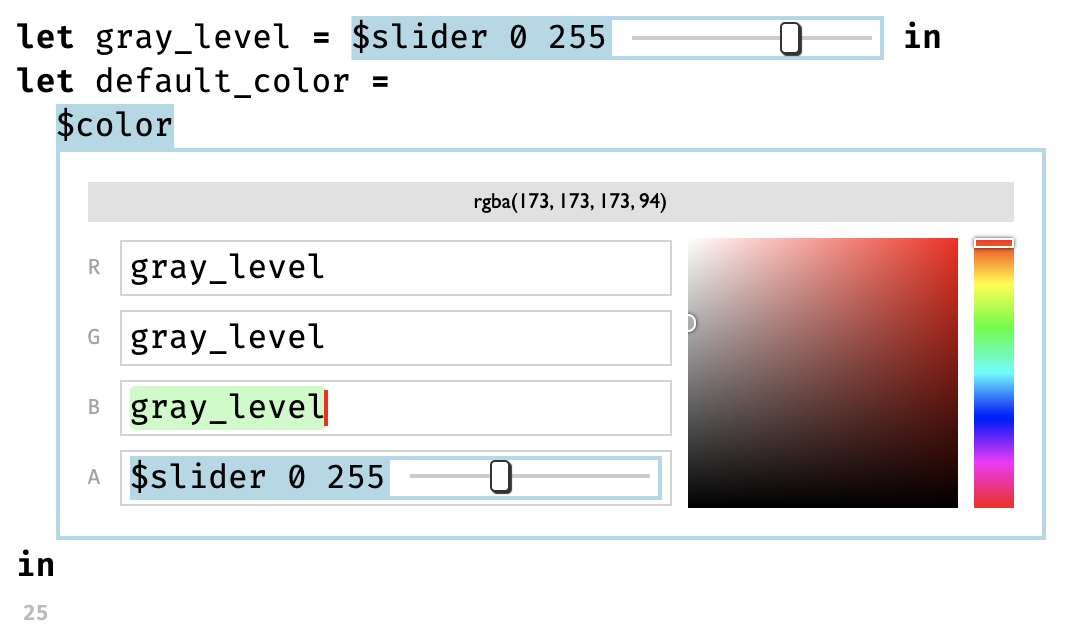
\includegraphics[width=\linewidth]{slider-color-livelits.png}
    \end{subfigure}
  \end{minipage}
  \hspace{10.5mm}
  \begin{subfigure}[t]{0.50\textwidth}
  \begin{snugshade}
   \vspace*{-2mm}
    \caption{\textbf{Case Study}: Grading with Livelits}
    \label{fig:grading}
    \vspace*{1mm}
     \end{snugshade}
    \vspace*{-1mm}
    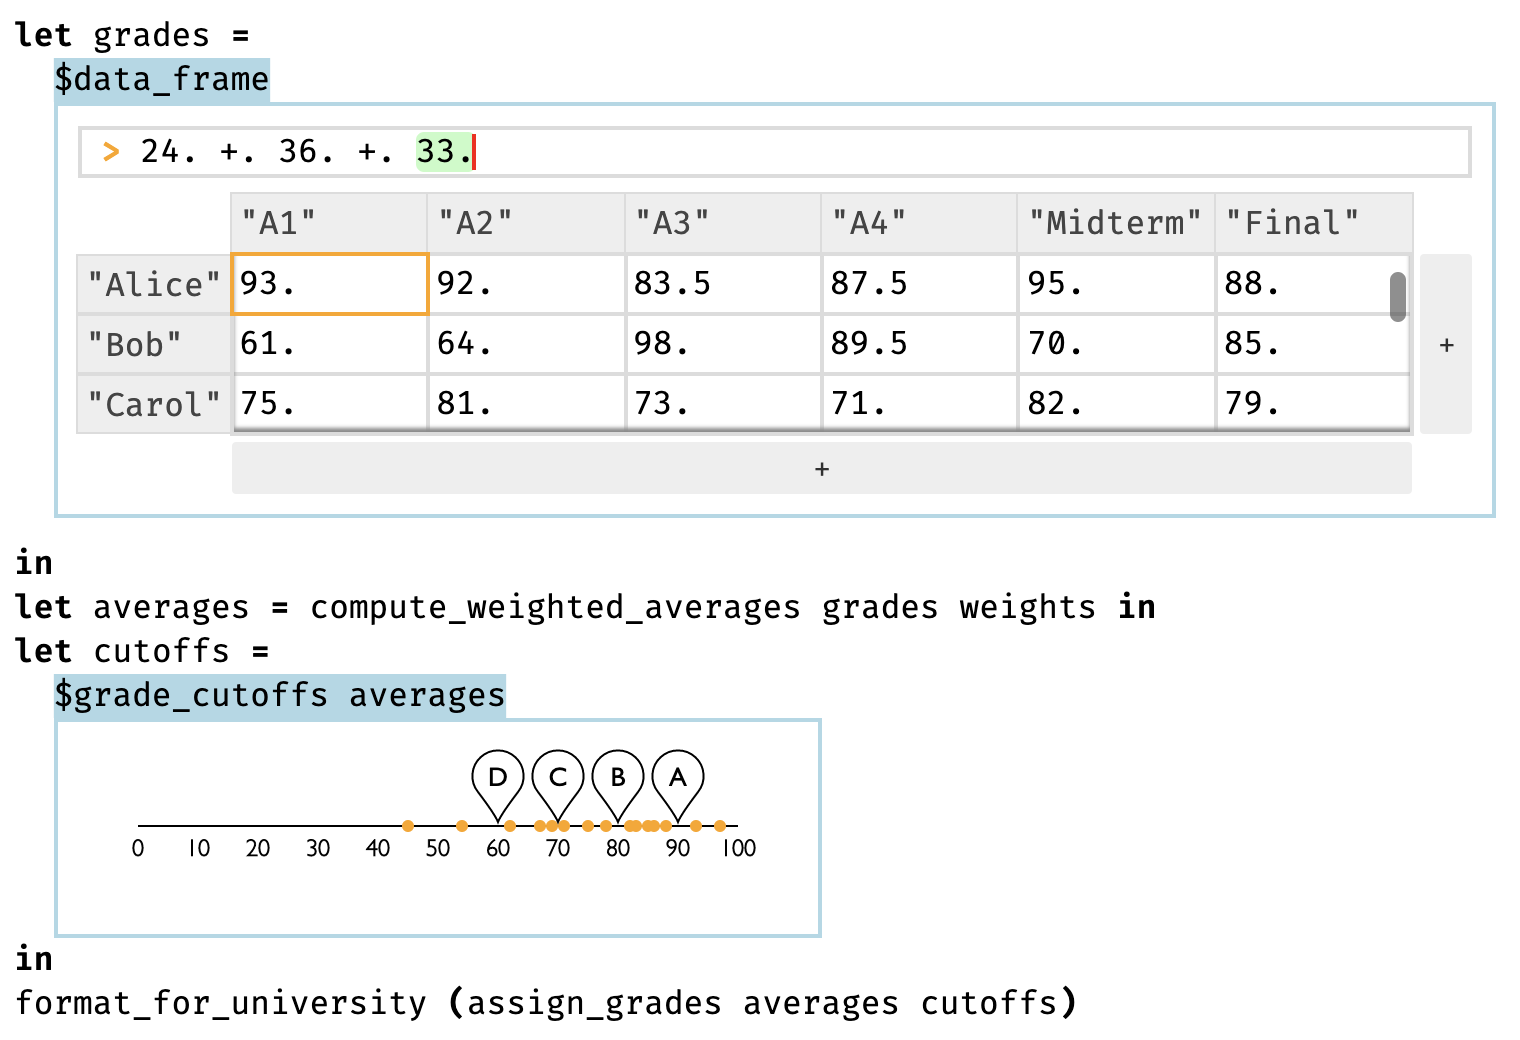
\includegraphics[width=\linewidth]{grade-cutoff-livelit.png}
  \end{subfigure}
  \vspace{-4mm}
   \caption{Introductory Examples}
%   \vspace*{-2mm}
\end{figure*}

Of course, we are not the first to integrate direct manipulation interfaces
into symbolic programming environments.
% Prior work on projectional editing
% and active code completion, detailed in Sec. \ref{sec:related-work},
% has also considered the problem of entering expressions
% of certain types, like \li{Color},
% using specialized GUIs integrated into a program editor.
% We detail prior work in Sec.~\ref{sec:related-work}, but 
The prior work most relevant to this paper is the {Graphite} system for Eclipse for Java,
demonstrated in Fig.~\ref{fig:graphite} \cite{Graphite}.
Graphite allows a library provider to associate a GUI, called a \emph{palette}, with a type 
(via a Java class annotation).
Wherever an expression of this type is needed,
i.e. wherever there is a \emph{hole} of that type in the program
(as determined by Eclipse's online parser and typechecker),
the environment offers the client the option, via the code completion menu,
to interact with the palette.
Once the interaction is finished, the palette generates a
Java expression to fill the hole.
Figure~\ref{fig:graphite}, adapted from this prior work, demonstrates a color palette invoked using Graphite.
When the user presses the \li{Enter} key, the Java expression \li{new Color(173, 173, 173, 85)} is inserted at the cursor and the palette disappears.
Several related systems, such as the  
\textbf{mage} system for the Jupyter notebook environment \cite{DBLP:conf/uist/KeryRHMWP20}
behave fundamentally similarly.
Projectional editing, the visual macro system in Racket \cite{interactive-visual-syntax}, and a number of other designs
also confront this general problem of integrating GUIs and code.

\citet{Graphite} evaluated Graphite by surveying 473 developers 
and \citet{DBLP:conf/uist/KeryRHMWP20} evaluated \textbf{mage} by interviewing 9 developers.
Both studies found that
participants viewed the proposed mechanism favorably and 
would use a suitable GUI some or all of the time.
% \footnote{When presented with a color palette,
% many participants remarked that they rarely entered colors directly into Java code,
% but rather into stylesheets.
% Other palettes, e.g. a palette
% that supported regular expression construction, were viewed as more
% suitable for Java code.
% The mechanisms being considered are suitable both for general-purpose languages
% and typed domain-specific languages like typed stylesheets, which can often be embedded into modern
% general-purpose languages.}
This and other prior work also collectively showcase a wide variety of use cases \cite{Graphite,DBLP:conf/uist/KeryRHMWP20,interactive-visual-syntax}, 
and the Graphite survey solicited dozens of additional use cases from participants,
which the authors systematically taxonomize \cite{Graphite}. 
We take these extensive empirical findings   
as evidence for, and a showcase of, 
the value of this class of mechanisms for integrating GUIs into code.
\vspace{-1mm}
\subsection{Contributions}
\label{sec:contributions}
We turn our attention in this paper to several fundamental technical
deficiencies that limit GUI providers and clients using these prior systems.
To address these, 
we introduce a system of \emph{live literals}, or \emph{livelits}, 
demonstrated in Fig.~\ref{fig:color}. 
Livelits are unique in achieving all of the following properties.
(We describe which subset of these properties 
are achieved by prior systems,
including those just mentioned, 
in Sec.~\ref{sec:related-work}.)

\newcommand{\llproperty}[1]{\vspace{5px}\noindent\textbf{#1}.}

\llproperty{Decentralized Extensibility}
    Providers define livelits in libraries, and 
    clients invoke livelits by name. Livelit names, e.g. \li{\$color},  are prefixed by \li{\$},    
    to distinguish them from variables.
    % We call this \emph{decentralized extensibility}.
    % Both mage and Racket's visual syntax system are similarly extensible, 
    % but 
    % In Graphite, palettes are associated with class definitions, 
    % so there is a tighter association between 
    % Other systems, discussed in Sec.~\ref{sec:related-work}, 
    % are either non-extensible, or cannot be extended by library providers 
    % (only by, for example, separately installed editor extensions, or by 
    % regenerating the editor using a language workbench.)
 
\llproperty{Persistence}
  % In Graphite and \textbf{mage}, GUIs are {ephemeral},
  % i.e. they disappear after the initial interaction,
  % leaving behind only the generated textual code.
  % Only the programmer that initially enters the expression
  % benefits from the feedback and affordances that the GUI provides.
  % %
  % \footnote{Graphite does include an \emph{ad hoc} mechanism that
  % allows palettes to parse the code that is selected in the editor
  % when the palette loads, but this requires that each palette implement
  % a parser for the subset of Java used in the code that it generates,
  % and therefore this mechanism is quite brittle. It is also difficult
  % to persist GUI state that is not included in the generated code.}
  Livelits are persistent elements of the syntax tree. They operate as  
  graphical literals, rather than as the ephemeral code generation GUIs of Graphite and \textbf{mage}. 
  We define a pure model-view-update-expand architecture
  (a variation on Elm's model-view-update architecture \cite{ElmArchitecture}) 
  where only the model needs to be persisted.
  The dynamic meaning of a livelit is determined by macro expansion.
  % We chose the word ``literal'' rather than ``palette'' because,  persistence, livelits
  % operate as graphical literals.

\llproperty{Hygienic Composition}
% Prior systems have limited or no support for {entering sub-expressions within the GUI}, 
% so they are useful mainly for generating expressions composed of constants,
% e.g. color constants in Fig.~\ref{fig:color}(a).
%
  Livelits support sub-expressions directly in the GUI, which we call \emph{splices} (after
   \citet{TLMs}).
  Fig.~\ref{fig:color} demonstrates splicing: the RGBA components  
  are splice editors, so the client can define a variable, \li{baseline},
  to relate the color components 
  and use a slider livelit inline to specify the alpha component.
  % Similarly, Fig.~\ref{fig:grading}(b)\todo{subfigure labels}{} demonstrates a 
  %  data table livelit where each entry is a splice.
  
  Crucially, composition is strictly 
  governed by a hygiene discipline that ensures
  (1) \textbf{capture avoidance}, i.e. that variables that the client uses in splices 
  will not capture expansion-internal bindings; and 
  (2) \textbf{context independence}, i.e. that the livelit 
  can be invoked in any program context.%without pre-condition or conflict.

\llproperty{Parameterization} Livelits can form parameterized families.
  For example, \li{\$slider} in Fig.~\ref{fig:color} is parameterized by the slider's bounds.
  Parameters operate like splices, differing in that they can be partially applied in
  livelit abbreviations. For example, Fig.~\ref{fig:color}
  partially applies \li{\$slider} to \li{0} and \li{100} to define a \li{\$percent} slider.
  % \begin{lstlisting}[numbers=none]
  % let $percentage = $slider 0 100 in ...
  % \end{lstlisting}
  % Parameterization also underlies the hygiene mechanism, as we will discuss in Sec.~\ref{sec:livelit-definitions}.

\llproperty{Typing} Each livelit specifies the type of expansions it generates, 
and parameters and splices also specify types, 
so livelits are compatible with type-driven methodologies and tools.
Together with the hygiene discipline, this allow clients to reason abstractly about expansions, i.e.  
without inspecting the expansions or livelit implementations directly.

\llproperty{Liveness} Uniquely, livelits can evaluate splices 
  throughout the editing process 
  (i.e. in a \emph{live} manner \cite{DBLP:conf/icse/Tanimoto13}) 
  to provide feedback related to run-time behavior.
  For example, in Fig.~\ref{fig:color}, 
  displaying the selected color requires evaluating the RGBA
  component splices to numeric values.
  Evaluation occurs in a run-time environment (i.e. closure) determined by
  leaving the hole being filled by the livelit temporarily unfilled and then evaluating
  using a two-phased variant of the semantics for 
  live programming with typed holes developed by \citet{HazelnutLive}.
  We support live evaluation even for livelits 
  that appear inside a function. Multiple function calls lead 
  to multiple closures that the client 
   can select between.

\paragraph{Outline.} We begin in Sec.~\ref{sec:case-studies} by introducing
livelits from the perspective of client programmers. 
Our examples are organized into case studies 
and are chosen to demonstrate the novel contributions of this paper.
In Sec.~\ref{sec:livelit-definitions}, 
we consider the livelit provider's perspective by introducing livelit
definitions with a detailed example.
In Sec.~\ref{sec:livelit-calculus}, we define the \emph{typed livelit calculus}. 
We have mechanically specified the central mechanism, livelit expansion, and proven the associated metatheorems in Agda.
This calculus 
serves to capture the essential nature of livelits 
independent of the particularities of syntax, GUI frameworks, 
and other orthogonal design details,
because we believe livelits can be integrated into a wide variety of programming systems. 
In Sec.~\ref{sec:implementation}, we provide a more detailed account of our two implementations of livelits.
Our primary implementation, used in the screenshots in the paper,
is integrated into Hazel, a live programming environment designed 
around hole-driven development. 
We have also prototyped livelits within a standard text editor. 
Additionally, we discuss factors that must be considered when integrating livelits into languages with side effects.
In Sec.~\ref{sec:related-work}, we compare livelits to related work using the design properties outlined above 
as a rubric.
Finally, we conclude in Sec.~\ref{sec:discussion} after a discussion of present limitations and future work.
\section{Livelits by Example}\label{sec:case-studies}


In this section, we will detail the livelits mechanism by way of  
two domain-specific case studies:
a course grade assignment case study in Sec.~\ref{sec:live-grading}
and an image transformation case study in Sec.~\ref{sec:image-transformation}.
% We also briefly mention several other examples in Sec.~\ref{sec:additional-examples}.\todo{do we?}{}
These case studies have been implemented
in Hazel, a browser-based live programming environment for a dialect of Elm. 
Elm is an industrial pure typed functional language in the
ML family used for client-side web development. 
We assume basic familiarity with ML.

\subsection{Case Study: Grading with Livelits}\label{sec:live-grading}
Consider this familiar scenario: an instructor needs
(1) to record numeric grades for various assignments and exams, and
(2) to visualize and perform various computations with these numeric grades
in order ultimately to assign final letter grades.
(In fact, this case study is not contrived: one author is using Hazel to compute grades this semester.)

The most common end-user application for this task is the spreadsheet, because 
it allows the instructor to record grades using a natural tabular interface,
visualize this data in one of a finite number of plot styles, 
and perform basic computations,
with results updated live.
However, these affordances are limited. 
It is difficult to package up common operations 
into reusable libraries, interact with the data using domain-specific visualizations,
and perform complex, unanticipated operations 
(e.g. preparing the data in an idiosyncratic format demanded by the university's grading system).

General-purpose programming languages 
can handle these scenarios, but users 
lose the ability to receive live feedback and  
directly manipulate data and visualizations in the editor.

Livelits are able to address this tension.
Fig.~\ref{fig:grading}(c)\todo{sublabels} shows a Hazel program where 
the instructor alternates between programmatic and direct manipulation in several situations.

First, the instructor defines a value \li{grades} 
that records the grades for each student using a livelit, \li{\$dataframe}, 
that implements a tabular user interface. The formula bar 
allows the selected cell to be filled with an arbitrary Hazel expression. 
For the sake of demonstration, we show a cell that has been filled using another livelit, 
\li{\$slider}, in combination with symbolic manipulation.\todo{do this?}{}
The table itself displays not the expression itself but rather its value, just as in a spreadsheet.

Next, the instructor computes \li{averages} 
for each student by applying \li{compute_averages}, a helper function 
defined in a library  (not shown) shared between multiple courses.

Next, the instructor wants to ``eyeball'' reasonable \li{cutoffs} between letter grades 
by directly manipulating a domain-specific livelit, \li{\$grade_cutoffs}, that provides draggable ``paddles'' 
superimposed on a live visualization of the distribution of \li{averages}, which is provided as a livelit parameter.
% The value of \li{cutoffs} is a labeled 4-tuple containing each cut-off. 

Finally, 
the instructor programmatically assigns grades to students 
based on these \li{cutoffs} 
by calling \li{assign_grades} 
and \li{format_for_university},
again shared functions.

\subsection{Livelit Expansion}\label{sec:livelit-expansion}
Livelit invocations 
expand to expressions.
For example, the expansion of Fig.~\ref{fig:grading}(c) is:

\begin{lstlisting}[xleftmargin=0.2cm]
let grades = Dataframe (
  ["A1", "A2", "A3", "Midterm", "Final"],
  [("Alice", [24. +. 36. +. 33., 
              92., 83.5, 95., 88.]),
   ("Bob", [61., 64., 98., 70., 85.]),
   ("Ciri", [75., 81., 73., 82., 79.]),
   (* ... *) ]) in
let averages = compute_averages grades weights in
let cutoffs = (.A 90., .B 80., .C 70., .D 60.) in
format_for_university 
  (assign_grades averages cutoffs)
\end{lstlisting}

The client can inspect this expansion in Hazel via a toggle (not shown).
Ideally, however, reasoning about types and binding
should not require the client to inspect the expansion 
nor the livelit implementation (which specifies the expansion logic 
as we will describe in Sec.~\ref{sec:livelit-definitions}).
After all, function clients do not need to look inside
function bodies to reason about types and binding.
Instead, in the words of \citet{DBLP:conf/ifip/Reynolds83},
``type structure is a syntactic discipline for maintaining levels of abstraction''.
Livelits maintain this discipline by
several means, described next in Sec.~\ref{sec:expansion-typing}-\ref{sec:hygiene}.

\subsubsection{Expansion Typing} 
\label{sec:expansion-typing}
To support abstract reasoning about the type of the expansion,
livelit definitions declare an \emph{expansion type}.
The declarations of the livelits in Fig.~\ref{fig:grading},
eliding their implementations, are:
\begin{lstlisting}[numbers=none,xleftmargin=0cm]
livelit $dataframe at Dataframe {...}
livelit $grade_cutoffs(averages: List(Float)) at 
  (.A Float, .B Float, .C Float, .D Float) {...}
livelit $slider (min: Int) (max: Int) at Int {...}
\end{lstlisting}
The expansion type of \li{\$dataframe} is \li{Dataframe},
which classifies tabular floating point data together with string row and column names (see the expansion above).
The expansion type of \li{\$grade_cutoffs} is a labeled product of grade cutoffs (field labels are written \li{.label}
rather than \li{label:} in Hazel).
Hazel displays the information in the livelit declaration when the cursor is on the livelit's name,
just as it displays typing information in other situations (not shown).\todo{cite HATRA}{}

\subsection{Compositionality}\label{sec:splicing-and-parameterization}
Livelits are compositional: they can work with sub-expressions  
in the form of parameters and splices.

\subsubsection{Parameters}\label{sec:parameterization} 
Livelit can declare a finite number of parameters of specified types. 
For example, \li{\$grade_cutoffs} above declares one parameter,
the averages to be plotted, of type \li{List(Float)}.
Parameters are applied  
using function application notation 
as seen in Fig.~\ref{fig:grading}(c) or 
using the pipelining (i.e. reverse function application) operators, \li{<|} and \li{|>}, 
which allow multiple livelits to form dataflows (not shown).

Livelit abbreviations can partially apply parameters. For example, 
we can partially apply the first parameter of \li{\$slider} to define a parameterized unsigned slider livelit:
\begin{lstlisting}[numbers=none,xleftmargin=0cm]
let $uslider = $slider 0 in ...
\end{lstlisting}
Only livelits with no remaining parameters can be invoked, 
so writing \li{\$uslider} in expression position will display as a ``missing livelit parameter'' error.%
\footnote{\label{footnote:typing}In Hazel, erroneous expressions 
are automatically placed inside holes so that they do not prevent other parts of the program from evaluating
\cite{HazelnutLive}.}


\begin{figure*}
  \begin{center}
    \begin{subfigure}[t]{0.5\textwidth}
      \centering
      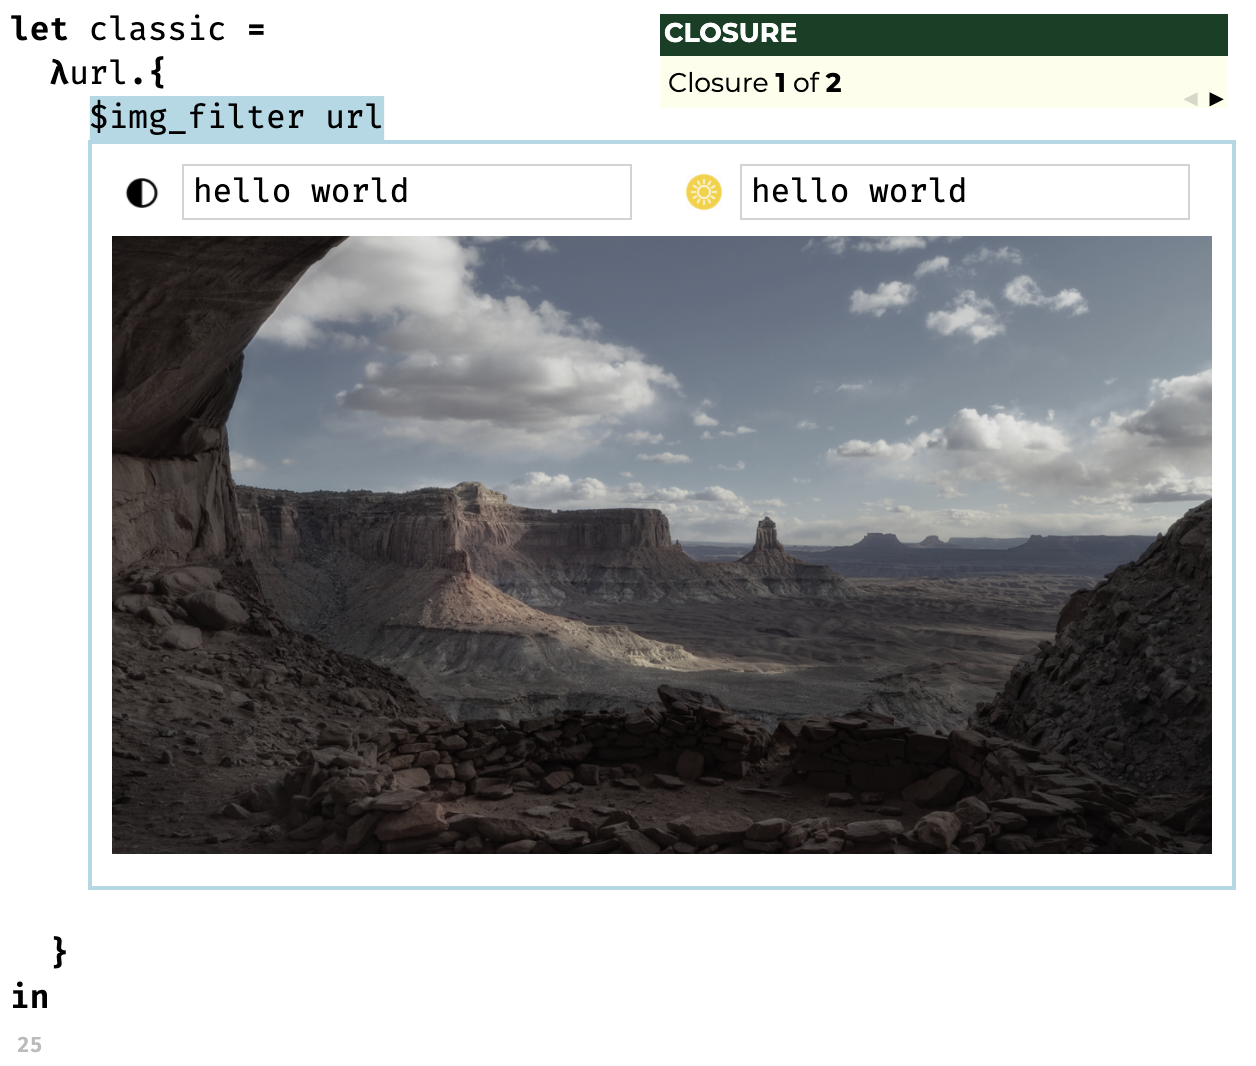
\includegraphics[width=15pc]{img-filter-1.png}
      \caption{}
    \end{subfigure}\begin{subfigure}[t]{0.5\textwidth}
      \centering
      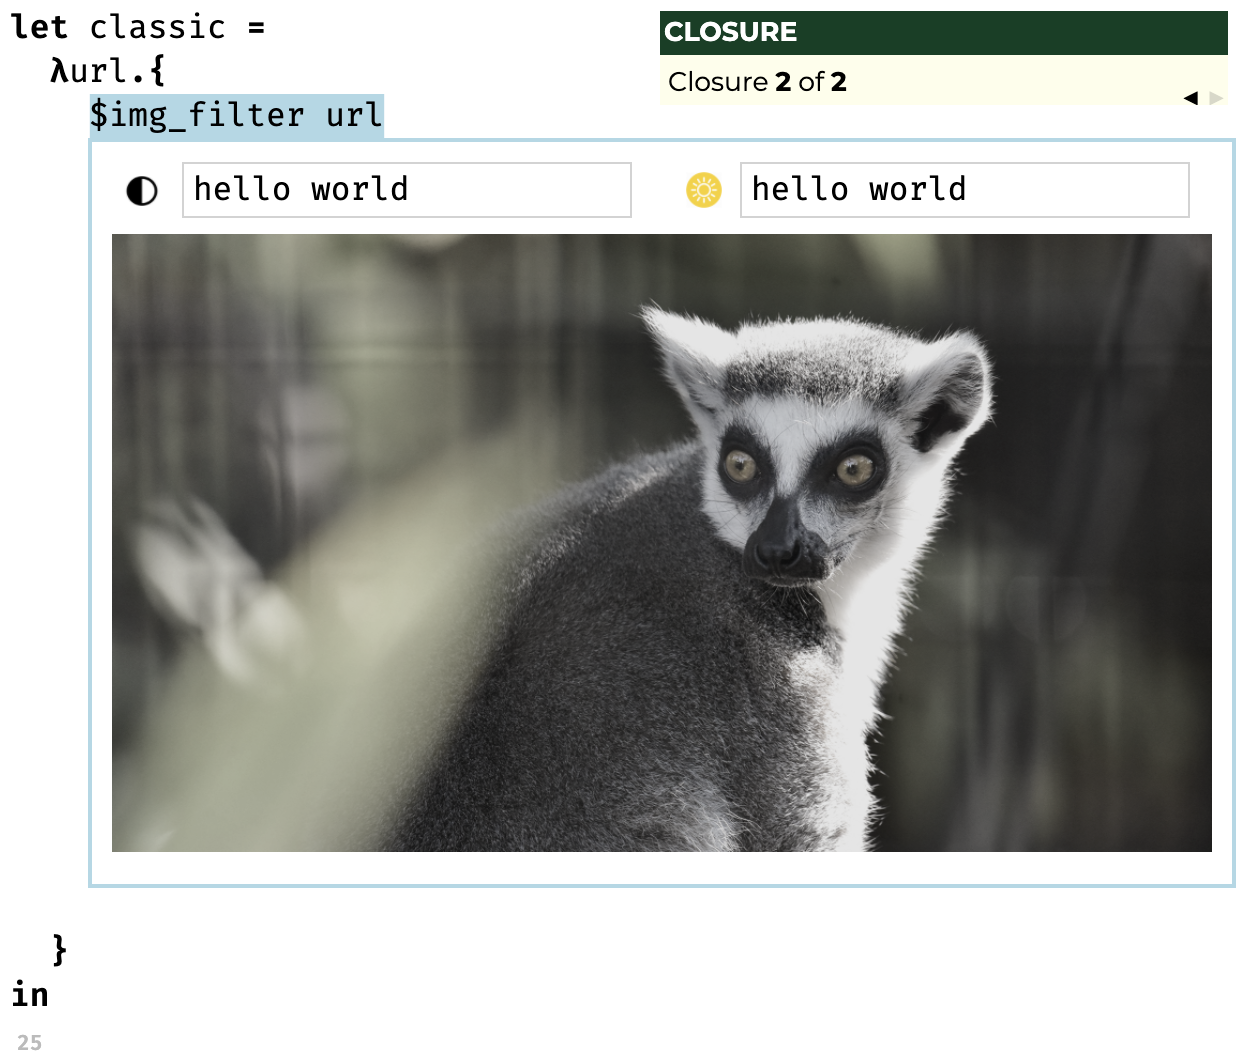
\includegraphics[width=15pc]{img-filter-2.png}
      \caption{}
    \end{subfigure}
  \end{center}
  \caption{Case Study: Image Transformation. The image shown is determined based on the selected closure.}
  \label{fig:img-transformation}
\end{figure*}


\subsubsection{Splices}\label{sec:splices}
Spliced expressions, or \emph{splices}, appear directly inside the livelit GUI.
Splices can be filled with Hazel expressions of any form, including other livelit invocations.
For example, each cell in the \li{\$dataframe} GUI in Fig.~\ref{fig:grading}
has a corresponding splice. The formula bar at the top 
allows the user to edit the splice corresponding to the selected cell,
and all of Hazel's editing affordances are available when the client does so.
% Not all splices necessarily appear in the GUI.
Unlike parameters, the number of splices can change 
as the user interacts with the livelit, e.g. when changing the number of rows or columns in a \li{\$dataframe}.
% The cell itself displays the live value of the spliced expression---
% (we return to live evaluation in Sec.~\ref{sec:live-evaluation} below.

The livelit provides an expected type for each splice when it is created.
For example, the splices for the row and column keys in Fig.~\ref{fig:grading}(c)\todo{go through subfigures}{} have expected type \li{String}, 
and the remaining cells have expected type \li{Float}.
Hazel surfaces and uses the expected type when the cursor is in the splice.\todo{cite HATRA paper}{}
% If an expression of invalid type is entered, it will display in an error hole as usual,
% and in Hazel this will not prevent evaluation of other expressions (see Footnote \ref{footnote:typing}).

% Unlike parameters, the number of splices is not fixed in the livelit declaration. Splices can be created,
% deleted, and filled through user interaction with the livelit. For example, clicking the \li{+} buttons
% in Fig.~\ref{fig:grading} will create new rows or columns, which will in turn generate new splices.

\subsubsection{Hygienic Composition}\label{sec:hygiene}
 

Ensuring that clients can reason about binding while leaving expansions
 invisible 
 requires a hygiene discipline that enforces \emph{capture avoidance}
and \emph{context independence} \cite{TLMs}\todo{cite michael hygiene paper}.

\textbf{Capture Avoidance.}
Splices and parameters can appear anywhere in the expansion. 
This becomes problematic when
they appear under a binder, e.g. in the body of a function or \li{let} binding.
Na\"ively, this could cause inadvertent capture of the bound variable by a free variable
in the parameter or splice. For example, consider a livelit that generates an expansion
of the following seemingly innocuous form:
\begin{lstlisting}[numbers=none]
let len = strlen <splice1> in
Some (<splice2> + len)
\end{lstlisting}
Here, \li{<splice2>} appears under the binding of \li{len}. If the client has filled
\li{<splice2>} with an expression that refers to a client-side binding of \li{len},
these references would na\"ively be captured. This would not occur in \li{<splice1>}, 
because the \li{let} is not recursive.
This breaks abstraction and is notoriously difficult to debug,
both for the livelit provider, who has no way to predict which variables a client will use,
 and the client, who does not know which variables the provider used.

To avoid this situation, parameters and splices are placed in the expansion
in a capture-avoiding manner: variables in splices
always refer to the bindings visible to the client, 
rather than bindings that are hidden inside the expansion.
We discuss how this is implemented in Sec.~\ref{sec:expansion}.
% This is implemented by alpha-renaming bindings internal to the expansion as necessary.
% (We discuss potentially relaxed variations of this hygiene discipline in Sec.~\ref{sec:discussion}.)

\textbf{Context Independence.}
The example expansion above used a library function, \li{strlen}.
Na\"ively, this expansion would break if placed 
in client contexts where \li{strlen} is not bound, or bound to 
an unexpected value.
To avoid requiring clients to determine and satisfy these invisible 
dependencies, the livelits mechanism enforces \emph{context independence}:
generated expansions are valid in any context. Dependencies are bound 
relative to the livelit definition site (see Sec.~\ref{sec:expansion}).

\subsection{Live Evaluation}\label{sec:live-evaluation}
Livelits have the ability to evaluate a splice or a parameter 
in order to provide better feedback about run-time behavior to the client.
The \li{\$dataframe} livelit uses this facility to display
the evaluation result for each cell, like a spreadsheet.
The \li{\$grade_cutoffs} livelit uses this facility to plot the grades, which were 
passed in as a parameter, on the number line.

\subsubsection{Closure Collection} The subtlety is that 
evaluation in Hazel is defined for closed expressions as usual,
but parameters and splices can be open, i.e. refer to surrounding variables. 
To provide a environment that binds these variables, 
Hazel performs \textbf{closure collection} in two phases.

In the first phase, \emph{proto-closure collection}, 
Hazel replaces each livelit with a uniquely numbered hole and then evaluates the program 
using the semantics for evaluating programs with holes developed by \citet{HazelnutLive}.
Evaluation proceeds around these holes, producing a result containing 
corresponding hole closures, i.e. holes with environments.

For example, there is one closure for \li{\$dataframe} in Fig.~\ref{fig:grading}.
It contains the value of \li{q1max}\todo{what?}{} and the other variables in scope. 
These values can be used to evaluate 
splices that use the corresponding variables, such as the cell selected in Fig.~\ref{fig:grading}(c). 

Similarly, the closure for \li{\$grade_cutoffs} in Fig.~\ref{fig:grading} includes 
the necessary \li{averages} variable, but 
its value depends on \li{grades}, which is determined by \li{\$dataframe}. 
If we stop after proto-closure collection,
then no useful value will be available:
the result will be \emph{indeterminate}, because \li{\$dataframe} has been replaced with a hole \cite{HazelnutLive}.
For this reason, there is a second phase of closure collection, called \emph{closure resumption}, 
where any livelit holes that appear
in the collected livelit closures are \emph{resumed}, i.e. the expansion is generated
(in this case, for the \li{\$dataframe} livelit) and evaluation resumes.
% Livelit expansions do not contain livelits, so no subsequent expansion / resumption phases are necessary.

% Hazel does not need to evaluate the program multiple times in order to support live closure collection
% as well as the usual live evaluation services it offers, because the final evaluation result 
% can also be determined by resumption.
% (We discuss how to address subtleties that arise 
% in the presence of non-commutative side effects in Sec.~\ref{sec:calculus-closure-collection}.)

\subsubsection{Indeterminate Results}
Even after resumption, some elements of the closure may remain indeterminate, e.g. due to holes that 
are not filled with livelits. 
When a livelit requests an evaluation result, it must be able to handle these indeterminate results.
For example, if there were missing grades,
then \li{\$grade_cutoffs} would have degraded functionality: 
it would display only the list elements that are values on the timeline, skipping indeterminate elements.
We will return to how this occurs in Sec.~\ref{sec:live-evaluation-def}.



\subsubsection{Case Study: Live Photo Filters}\label{sec:image-transformation}
\todo{revise this once we have final figure}{}
Closure collection can produce multiple closures when, for example, 
a livelit appears inside a function applied multiple times. 
Our next case study, in the photography domain,
demonstrates how Hazel handle this situation, and 
the workflow it enables. 

We interviewed a photographer 
who described a typical workflow: 
they use the Lightroom application to 
apply a set of adjustments and filters 
across all photos in a collection before making 
individual adjustments. 
Many photographers do this one photo at a time,
though this photographer had recently learned how to
use Lightroom's saved presets to 
apply adjustments to multiple photos at once.
However, they remained dissatisfied by the workflow.
They wanted to be able to see how the shared settings affected 
multiple photos as they tweaked them, without having to 
save and apply the preset repeatedly.
They also wanted to be able to change the shared settings
even after making certain individual adjustments.
They also expressed interest in defining parameterized 
presets, and in automating the process of 
posting sets to a website and social media. 

% For our next case study, we 
% developed a library of 
% image transformation livelits, 
% motivated by a desire to automate 



% The livelits we have considered so far generate simple values.

Motivated by this interview, 
we prototyped a collection of image transformation livelits.
One of these, \li{\$something} is demonstrated in Fig.~\ref{fig:img-transformation},
within a function, \li{classic_look}, that serveas as a ``preset'' that is 
mapped over a list of images (loaded by URL) at the bottom of the figure. 
% We show two for space reasons.

...\todo{finalize?}{}
This livelit takes 
a URL to an image as a parameter, and contains two splices of type \li{Int},
one to adjust the contrast, and the other to adjust the brightness.
In this example, we have filled those splices with a \li{\$slider}, but 
as above we could enter any expression of type \li{Int}, e.g. 
an arithmetic expression or a variable. 
The livelit shows a live preview of the transformed image.
The expansion generates the necessary calls to an image processing library, 
not shown.

Because the livelit appears inside a function applied (by \li{map}) twice, 
there are now two closures associated with the livelit. 
Rather than disabling live evaluation in situations like 
this, Hazel instead allows the programmer to select between the closures when 
the cursor is on the livelit expression via a simple sidebar toggle. 
This causes the view to change as shown in ...\todo{todo}{}
The live feedback is based on the selected closure.
This makes it easy to see how the image filter being designed here will affect a
number of example images by quickly toggling between closures. 
The underlying expansion remains abstract, i.e. it refers to the image via the \li{url} variable.

We showed this and similar examples to the photographer we had interviewed. 
They expressed substantial interest in this approach despite having only 
limited programming experience (with Python). They made the fair point that it 
would take substantial effort to match Lightroom's breadth of filters and effects, 
but with sustained effort, they agreed that this approach could be more powerful than 
Lightroom's point-and-click interface while retaining many of its benefits (specifically
mentioning the graphical sliders). Although this was only a single interview,
it is consistent with the body of evidence summarized in Sec.~\ref{sec:background}.

% \subsection{Additional Examples}\label{sec:additional-examples}
% It would be nice to have a gallery-style figure and a brief overview of some other case studies
% and how they exercise the novel features of the livelits mechanism. Maybe some statistics on how
% many lines of code it took.

% Ideas:
% \begin{itemize}
%   \item derivation trees like Joomy's system (\url{https://joom.github.io/proof-tree-builder/src/})
% \end{itemize}
\section{Livelit Definitions}\label{sec:livelit-definitions}

\begin{figure}
\begin{lstlisting}[xleftmargin=0.2cm]
type Color = (.r Int, .g Int, .b Int, .a Int)
livelit $color at Color {
  type Model = (.r SpliceRef, .g SpliceRef, 
                .b SpliceRef, .a SpliceRef)

  context { }

  let init : UpdateCmd(Model) = do 
    r <- new_splice(`Int`, Some(`0`))
    g <- new_splice(`Int`, Some(`0`))
    b <- new_splice(`Int`, Some(`0`))
    a <- new_splice(`Int`, Some(`100`))
    return (r, g, b, a)

  type Action = 
  | ClickOn(Color)

  let view : Model -> ViewCmd(Html(Action)) = 
    fun model -> do 
      (* determine a color to display *)
      r_res <- eval_splice(model.r)
      g_res <- eval_splice(model.g)
      b_res <- eval_splice(model.b)
      a_res <- eval_splice(model.a)
      let cur_color : Color = 
        case (r_res, g_res, b_res, a_res) 
        | (Some(Val(IntLit(r))), 
           Some(Val(IntLit(g))), 
           Some(Val(IntLit(b))), 
           Some(Val(IntLit(a)))) -> 
             Some((r, g, b, a))
        | _ -> 
          (* indeterminate color shown as X *)
          None 
      in 
      
      (* generate splice editors *)
      let size = FixedWidth(20) in 
      r_editor <- editor(model.r, size)
      g_editor <- editor(model.g, size)
      b_editor <- editor(model.b, size)
      a_editor <- editor(model.a, size)
      
      (* ... now we can render the UI ... *)
    
  let update : 
      Model -> Action -> UpdateCmd(Model) =
    fun model (ClickOn c) -> do 
      set_splice(model.r, IntLit(c.r))
      set_splice(model.g, IntLit(c.g))
      set_splice(model.b, IntLit(c.b))
      set_splice(model.a, IntLit(c.a))
      return model
  
  let expand : Model -> (Exp, List(SpliceRef)) = 
    fun model -> (`fun r g b a -> (r, g, b, a)`, 
      [model.r, model.g, model.b, model.a])
}
\end{lstlisting}
\vspace{-8px}
\caption{Livelit Implementation}
\label{fig:color-impl}
\end{figure}

\noindent
We will now take the perspective of a livelit provider.
Fig.~\ref{fig:color-impl}
defines \li{\$color} from Fig.~\ref{fig:color}, 
which is our prototypic example of a livelit 
definition. 
We omit certain  
incidental details and use unimplemented syntactic sugar, including
Haskell-style \li{do} notation \cite{marlow2010haskell} and quasiquotation \cite{bawden1999quasiquotation}, for presentation.

Livelit definitions are scoped and packaged like 
any other definition. Each \emph{definition} consists of a \emph{declaration} and an \emph{implementation}. 
In Hazel, a ``template'' declaration and implementation is generated 
as soon as the user types ``\li{livelit\ }''.

\subsection{Livelit Declarations} 
Line 2 of Fig.~\ref{fig:color-impl} is \li{\$color}'s declaration,
which defines its name and its {expansion type}, \li{Color}, defined on Line 1. 
Both are required. 
Livelit parameters can also optionally appear here as shown in the declarations in Sec.~\ref{sec:expansion-typing}. 
The declaration is part of the client interface, 
as discussed in Sec.~\ref{sec:expansion-typing}-\ref{sec:parameterization}. 

\subsection{Livelit Implementations}
The curly braces delimit the livelit's implementation, which is not intended to be seen 
by clients. Each livelit implementation must define types \li{Model} and \li{Action}, 
values \li{init}, \li{view}, \li{update}, and \li{expand} with the signatures specified in Fig.~\ref{fig:color}, 
and a \li{context}, which is a listing of definition-site bindings that the livelit can make use of as described below. All of these are included in the generated template.
 These constitute a variation on the pure functional model-view-update
architecture popularized by Elm \cite{ElmArchitecture}. We add a fourth component,
expansion generation. In addition, we use a monadic framework (\emph{a la} Haskell \cite{marlow2010haskell}) to provide a pure   
 interface between the livelit and the editor: monadic commands, like \li{new_splice} discussed below, are executed by the editor,
and \li{do} notation provides syntactic sugar for monadic bind.


\subsubsection{Model}\label{sec:model}
The state of a livelit's GUI is determined by its model value. 
Line 3 of Fig.~\ref{fig:color-impl} specifies the corresponding \emph{model type},
here a labeled 4-tuple of \emph{splice references}, one for each of the four splices
that appear in the GUI in Fig.~\ref{fig:color}.
The model is how the GUI state is persisted in the syntax tree, so 
 the system requires that the model type supports automatic serialization
 (so functions cannot appear in models).

The \li{init} value on Line 8 determines the value of the model
when the livelit is first invoked in the editor.
It is a command in the \li{UpdateCmd} monad, further discussed in Sec.~\ref{sec:def-update}, that returns the 
initial model value after generating four new splices 
using the \li{new_splice} command:
\begin{lstlisting}[numbers=none]
  new_splice : (Typ, Maybe(Exp)) 
               -> UpdateCmd(SpliceRef)
\end{lstlisting}
This command creates a splice
of the given type and, optionally, its initial contents. 
It returns a splice reference, which uniquely identifies that splice.
In this section, bolded types  
are defined in the standard library. The \li{Typ} and \li{Exp} types 
encode the syntax of Hazel's types and expressions 
and we use quasiquotation, e.g. \li{`0`}, as the introduction forms \cite{bawden1999quasiquotation}. 
% If no initial expression is provided, the splice starts as  
% an empty hole.

To ensure \emph{context independence}, 
the system checks that the splice type and initial content are valid 
assuming only the parameters and explicitly specified \li{context} on Line 6.
Here, the context is empty because \li{Int} is a built in type
and the initial expressions are integer literals. 
We use an explicit context, rather than implicitly capturing all bindings 
at the definition site, 
to ensure that private bindings are not unintentionally  
leaked to clients \cite{TLMs}.
% Formally, captured variables can be understood as parameters that have been 
% immediately partially applied.

\subsubsection{Action}
Line 15 defines the \li{Action} type for the \li{\$color} livelit, which 
specifies a single user-initiated action: clicking on a color using
the right half of Fig.~\ref{fig:color}. Actions are emitted
from event handlers (e.g. click handlers) defined in the computed \li{view}, Sec.~\ref{sec:def-view}, 
and actions are consumed by the \li{update} function, Sec. \ref{sec:def-update}, causing a change to the model.

\subsubsection{View}\label{sec:def-view}
The \li{view} function computes the view given the model and access to the commands in 
the \li{ViewCmd} monad (which is distinct from the \li{UpdateCmd} monad). The computed view is a value of type \li{Html(Action)}.  
This type  provides a simple immutable
encoding of an HTML element, where the type parameter is the type of actions that 
are emitted by event handlers that can be attached to elements, e.g.
\li{on_click} and so on. 
We elide the details of the particular user interface in Fig.~\ref{fig:color}, 
but note that livelit implementations can themselves invoke other  
livelits, e.g. the \li{view} function could use livelits for 
expressing user interface widgets and layouts (not shown). 
Instead, we focus on three mechanisms exposed by \li{ViewCmd}: live evaluation,
splice editors, and result rendering.


\paragraph{Live Evaluation}
\label{sec:live-evaluation-def}
As discussed in Sec.~\ref{sec:live-evaluation}, 
the view can depend on the result of evaluating a splice or a parameter
under the closure the client has selected.
(Parameters, not shown in this example but discussed in Sec.~\ref{sec:parameterization}, operate like splices and have type \li{SpliceRef}
within the livelit definition.)
The interface between the view and the live evaluator 
is via the 
following command:
% Actually, it can depend on an encoded function of 
% multiple splices as long as the function is well-typed using only the capture set, 
% under the closure that the client has selected using one of the following
% commands:
\begin{lstlisting}[numbers=none,xleftmargin=0cm]
eval_splice : SpliceRef -> ViewCmd(Maybe(Result))
\end{lstlisting}

%eval_fun : (Exp, List(SpliceRef)) -> ViewCmd(Maybe(Result))

The \li{None} case 
arises when evaluation is not possible, e.g. because no closures are collected 
or because no value has been collected for a variable used in the splice. 
In practice, there is an implicit hole at the end of each cell in Hazel, so 
livelits will have at least one closure containing results for at least 
the top-level bindings. Function argument values may not be available 
if that function has not been applied.
% because the free variables in the selected closure overlap with the free 
% variables in the provided expression. This occurs only when the user has selected
% a closure that appears under a binder in the evaluation result (e.g. because 
% the result is a lambda). 
% We discuss this further in Sec.~\ref{sec:calculus-closure-collection}.

If available, \li{Result} distinguishes two possibilities:
\begin{lstlisting}[numbers=none]
type Result = Val(Exp) | Indet(Exp)
\end{lstlisting}
The \li{Val} case arises when evaluation produces a value, whereas the 
\li{Indet} case arises when evaluation results in an indeterminate expression,
i.e. an expression that cannot be fully evaluated due to holes 
in critical positions \cite{HazelnutLive}.

Lines 26-34 determine a color to display in the color preview 
if all four splices evaluate to integers. Otherwise, there is not 
enough information to determine a color. The livelit 
indicates this situation by disabling the color preview.

Livelits can attempt to offer feedback even when the result is indeterminate,
because indeterminate expressions might nevertheless contain useful information.
For example, a livelit that previews a sequence of notes as audio might be able 
to handle a list of notes where certain notes are missing, i.e. holes, by 
playing silence.
This behavior is highly domain-specific, so each livelit provider must decide 
whether and how indeterminate results are supported.

\paragraph{Splice Editors}
The view includes an editing area for each splice. These editors must support all of 
Hazel's editing services. To support this, the \li{view} function
can request an editor with a given dimension (in character units) for a given splice:
\begin{lstlisting}[numbers=none]
editor : (SpliceRef, Dim) -> ViewCmd(Html(a))
\end{lstlisting}
The result is an opaque \li{Html(a)} value that the remainder of the function 
can place where needed. When the livelit is rendered, this part of the tree is 
under the control of Hazel. The \li{Dim} parameter currently supports only a fixed
character width, with overflow causing scrolling, but in the future we plan to offer 
to offer more flexible layout options.

\paragraph{Result Rendering}
Some livelit views needs to include 
a rendered evaluation result. For example, each of the cells in the \li{\$dataframe}
livelit in Fig.~\ref{fig:grading} show the evaluation result for the corresponding 
cell. Only the formula bar at the top is an editor. To support this, the \li{view}
function can use the \li{result_view} command, which mirrors the \li{editor} command:
\begin{lstlisting}[numbers=none]
result_view : (SpliceRef, Dim) 
              -> ViewCmd(Maybe(Html(a)))
\end{lstlisting}
\subsubsection{Update}\label{sec:def-update}
When the user triggers an event in a livelit view, it emits an \li{Action}.
The system responds by calling the \li{update} function to determine how 
this action should affect the model and, in some cases, the splices. 

% We discussed in Sec.~\ref{sec:model} that the \li{UpdateCmd}
% allows new splices to be generated in response to user actions. 
% For example, the \li{\$dataframe} livelit uses this when new rows
% or columns are added.

In Fig.~\ref{fig:color-impl}, we see that the \li{\$color} livelit responds to 
the \li{ClickOnColor} action by invoking the \li{set_splice} command to overwrite 
the current splices with integer literals determined based on which color the user
clicked on:
\begin{lstlisting}[numbers=none]
  set_splice : (SpliceRef, Exp) -> UpdateCmd ()
\end{lstlisting}
As with \li{new_splice} described in Sec.~\ref{sec:model},
the system maintains context independence by checking the expression against the splice type 
and only allows use of the specified \li{context}.

When the model is updated, a new view is 
computed. The system then performs a diff between the old and new view in order to 
efficiently perform the necessary imperative updates to the editor's visual state.
Changes to splices can also cause the view to be recomputed, because the view might 
evaluate the splices. The \li{UpdateCmd} monad does not itself 
have the ability to request evaluation (\li{eval_splice}), because the model should not depend directly  
on which closure the user has selected. 
Of course, the \li{view} might emit 
result-dependent actions when appropriate.

\subsubsection{Expansion}
\label{sec:expansion}
The ultimate purpose of a livelit is to fill the hole where it appears by generating an expansion,
i.e. an expression of the expansion type, here \li{Color}.
The \li{expand} function determines the expansion given the model. 
The two are necessarily distinct: the model encodes the GUI state, 
and so usually tracks ephemeral widget state, like which tab is active in a tabbed GUI, 
as well as splice references, which refer only indirectly to the spliced expressions themselves, discussed below. 
This information is not needed at run-time as part of the expansion.
Only the model is persisted when a Hazel program is saved, because the expansion 
can be regenerated by calling \li{expand} whenever needed.

The expansion can include spliced expressions, 
but the system does not make these expressions  
available directly as values of type \li{Exp}. 
Instead, the expansion must treat splices parametrically. 
In particular, \li{expand} returns an encoded \emph{parameterized expansion}, of type \li{Exp}, 
paired with a list of \li{SpliceRef}s (which can come from 
both splices and parameters as discussed above).
The {parameterized expansion}
  is a function 
 (here curried)
 that takes an argument for each listed \li{SpliceRef}. 
 That argument is of the corresponding splice 
type, which was provided when the splice was initialized. 
 The return type of the parameterized expansion is the expansion type.
 So here, the parameterized expansion for \li{\$color} must be a function of type 
 \li{Int -> Int -> Int -> Int -> Color} because the splices 
 in the splice list were each of type \li{Int}.


This parameterization strategy makes enforcing the binding discipline described in Sec.~\ref{sec:hygiene}
straightforward. 
Context independence is maintained by allowing the parameterized expansion 
to depend only on bindings given in the explicit \li{context}, which 
the system maintains bound relative to the definition site. 
The splices can 
depend only on the client site typing context. The use of function application ensures
that splices are capture avoiding. 
% We consider this more formally next.

Note that Hazel does \emph{not} statically check the definition of \li{expand}
to ensure that the encoded parameterized expansion has the necessary type in the specified \li{context}. Instead, the parameterized expansion 
is only \emph{validated} at each livelit invocation site, with errors reported to the client. 
A \emph{typed quotation} system as in, e.g., MetaOCaml \cite{DBLP:conf/flops/Kiselyov14}, could be adapted to allow for definition-site verification, as discussed in \cite{TLMs}, but 
note that   
the type of the quotation depends on the type of each splice in 
the splice list, which has arbitrary length in general (e.g. the 
number of splices in the \li{\$dataframe} livelit 
depends on how many rows and columns the user has added).

\section{A Simply Typed Livelit Calculus}\label{sec:livelit-calculus}

\begin{figure}
    \[
    \arraycolsep=3pt\begin{array}{rlcl}
        \mathsf{Typ} & \tau & ::= &
                                    % \tnum ~\vert~
                                    \tarr{\tau_1}{\tau_2} ~\vert~
                                    \tprod{\tau_1}{\tau_2} ~\vert~
                                    \tunit ~\vert~
                                    \tsum{\tau_1}{\tau_2} ~\vert~
                                    t ~\vert~
                                    \trec{t}{\tau}\\
        \mathsf{UExp} & \hat{e} & ::= & 
                                 x ~\vert~
                                 \hlam{x}{\hat e} ~\vert~
                                 \hap{\hat e_1}{\hat e_2} ~\vert~
                                 ... ~\vert~
                                %  \hpair{\hat e_1}{\hat e_2} ~\vert~
                                %  \hprl{\hat e} ~\vert~
                                %  \hprr{\hat e} ~\vert~
                                %  \htriv ~\vert~
                                %  \hinL{\hat e} ~\vert~
                                %  \hinR{\hat e} ~\vert~
                                %  \hroll{\hat e} ~\vert~
                                %  \hunroll{\hat e} \\
                                 \hehole{u} ~\vert~
                                 \haplivelit{u}{a}{\dtxt{model}}{\splices}\\
        \mathsf{EExp} & e & ::= & x ~\vert~ \hlam{x}{e} ~\vert~ \hap{e_1}{e_2} ~\vert~ ... ~\vert~ \hehole{u}\\
        \mathsf{IExp} & d & ::= & x ~\vert~ \hlam{x}{d} ~\vert~ \hap{d_1}{d_2} ~\vert~ ... ~\vert~ \dehole{u}{\sigma}\\
        \mathsf{Splice} & \psi & ::= & \hsplice{\hat e}{\tau}
    \end{array}
    \]
    \caption{Syntax of types, $\tau$, unexpanded expressions, $\hat{e}$, expanded expressions, $e$, and internal expressions, $d$.
    Here, $x$ ranges over variables, $u$ over hole names, and $\livelitname{a}$ over livelit names.
    We write $\splat{\psi_i}$ for a finite sequence of $n \geq 0$ splices,
    and $\sigma$ for finite substitutions of $n \geq 0$ internal expressions for variables, $[d_1/x_1, \cdots, d_n/x_n]$.
    We elide standard forms
    related to product, sum, and recursive types.
    }
    \label{fig:syntax}
    \end{figure}

In order to communicate the semantics of livelits
independently
of the specifics of the Hazel environment and the web platform, 
we now specify a simply typed \emph{livelit calculus}.

Fig.~\ref{fig:syntax} specifies the syntax of the livelit calculus.
Programs are written as \emph{unexpanded expressions}, $\hat e$, which are \emph{expanded} to
\emph{external expressions}, $e$, before being \emph{elaborated}
to \emph{internal expressions}, $d$, for evaluation. All three sorts are classified
by the same types, $\tau$. We include partial functions, products, sums, and recursive
types, all in their standard form \cite{pfpl}, but this specific type structure is not critical.
Any language expressive
enough to encode its own abstract syntax 
would be a suitable basis for a livelit calculus. 

We begin in Sec.~\ref{sec:external-and-internal-lang} with a terse
overview of the external and internal languages,
which are adapted from Hazelnut Live \cite{HazelnutLive}.
We then detail livelit expansion (Sec.~\ref{sec:calculus-expansion}) and 
liveness via closure collection (Sec.~\ref{sec:calculus-closure-collection}). 
% and parameterization (Sec.~\ref{sec:calculus-parameterization}).


\subsection{Background: External and Internal Language}\label{sec:external-and-internal-lang}
The external and internal languages are straightforward adaptations of the
external and internal languages of \emph{Hazelnut Live},
a typed lambda calculus that assigns static and dynamic meaning to programs with holes,
notated $\hehole{u}$ where $u$ is a \emph{hole name} \cite{HazelnutLive}.
We omit non-empty holes (which internalize type inconsistencies \cite{Hazelnut}) and type holes
(which operate like the unknown type from gradual type theory \cite{Siek06a,Hazelnut}).
These mechanisms are orthogonal to livelits and are included in our implementation.

External expressions, e, are governed by a typing judgement of the form, $\hasType{\Gamma}{e}{\tau}$,
where the typing context, $\Gamma$,
is a finite set of typing assumptions of the form $x : \tau$ \cite{pfpl}.

The internal language is a contextual type theory \cite{Nanevski2008}, i.e. the typing judgement is
of the form $\hasTypeD{\Delta}{\Gamma}{d}{\tau}$ where $\Delta$ is a finite set of hole typing
assumptions of the form $u :: \tau[\Gamma]$.
We need this hole typing context only for the internal language because, although hole names are assumed
unique in the external language, they can be duplicated during evaluation of internal expressions.
The hole context ensure that each closure associated with hole $u$, written $\dehole{u}{\sigma}$,
shares a type and can be filled
with expressions valid under a shared context.

\newcommand{\tnat}{\mathsf{nat}}

External expressions are given dynamic meaning by typed elaboration to internal expressions, $d$,
according to the judgement $\elabs{\Gamma}{e}{d}{\tau}{\Delta}$.
The main purpose of elaboration is to initialize the substitution $\sigma$ on each hole closure,
which operates to capture
the substitutions that have occurred around that hole during evaluation. The key rule is:
\begin{mathpar}
\inferrule[Elab-Hole]{ }{
    \elabs{\Gamma}{\hehole{u}}{\dehole{u}{\idof{\Gamma}}}{\tau}{u :: \tau[\Gamma]}
}
\end{mathpar}
The substitution is initially the identity substitution, $\idof{\Gamma}$, i.e. the
substitution that maps each variable in $\Gamma$ to itself, because no substitutions have yet occurred. For example,
\[ \elabs{ }{(\hlam{x}{\hehole{u}})~\hnum{5}}{(\hlam{x}{\dehole{u}{[x/x]}})~{\hnum{5}}}{\tnat}{u :: \tnum[x : \tnat]} \]


During evaluation, $\evalsTo{d}{d'}$, the closure's substitution accumulates the substitutions that occur. For example,
the internal expression above evaluates as follows:
\[
  \evalsTo{(\hlam{x}{\dehole{u}{[x/x]}})~{\hnum{5}}}{
      \dehole{u}{[\hnum{5}/x]}
  }
\]
% We will use hole closures to support live programming with livelits in Sec.~\ref{sec:calculus-closure-collection}.


All of these judgements are adapted directly from Hazelnut Live,
differing only in that we use a declarative rather than an algorithmic (bidirectional)
formulation for simplicity. Rather than restating the rules, we simply state the key governing
metatheorems and refer the reader to the prior work and our Agda mechanization (Sec.~\ref{sec:agda}) for the full details \cite{HazelnutLive}.

First, we have that elaboration preserves typing.
\begin{theorem}[Typed Elaboration]
    If $\hasType{\Gamma}{e}{\tau}$ then $\elabs{\Gamma}{e}{d}{\tau}{\Delta}$ for some $d$ and $\Delta$ such
    that $\hasTypeD{\Delta}{\Gamma}{d}{\tau}$.
\end{theorem}

Next, we have that evaluation of a closed expression with holes produces a final (i.e. irreducible) preserves typing.
\begin{theorem}[Preservation]
    If $\hasTypeD{\Delta}{\cdot}{d}{\tau}$ and $\evalsTo{d}{d'}$ then $\isFinal{d'}$ and $\hasTypeD{\Delta}{\cdot}{d'}{\tau}$.
\end{theorem}

\subsection{Expansion}\label{sec:calculus-expansion}

The novelty of the livelit calculus is entirely in its handling of unexpanded expressions,
$\hat e$, which are given meaning by typed expansion to external expressions,
$e$, according to the judgement $\expands{\Phi}{\Gamma}{\hat e}{e}{\tau}$
defined in Fig.~\ref{fig:expansion}.
Unexpanded expressions mirror external expressions but for the presence of livelit invocations.
The rules for the mirrored 
forms like variables and functions, both shown in Fig.~\ref{fig:expansion},
are simple.

\subsubsection{Livelit Contexts}\label{sec:livelit-contexts}

Livelit definitions are collected in the livelit context, $\Phi$, which
maps livelit names to livelit definitions of the following form:
\[ \livelitCtxEntry{a}{\taut{expand}}{\taut{model}}{\dtxt{expand}} \]
Here, $\taut{expand}$ is the expansion type, $\taut{model}$ is the model type,
and $\dtxt{expand}$ is the expansion function, which generates an expansion given a model.
We omit the logic related to view computations and actions, which are tied to a particular 
UI framework and have only indirect semantic significance.

% For a livelit context to be well-formed, we require that each livelit definition be well-formed.
% This in turn requires that the expansion function be hole-free and have the correct type.
\begin{definition}[Livelit Context Well-Formedness]
    A livelit context $\Phi$ is well-formed if and only if for each livelit definition,
    $\livelitCtxEntry{a}{\taut{expand}}{\taut{model}}{\dtxt{expand}} \in \Phi$,  we have
    $\hasType{}{\dtxt{expand}}{\tarr{\taut{model}}{\expType}}$.
\end{definition}
Here, $\expType$ stands for a type whose values isomorphically encode
external expressions. The isomorphism is mediated in one direction by
the encoding judgement $\encodeExp{e}{d}$ and the other by the decoding judgement $\decodeExp{d}{e}$.
Any scheme is sufficient, so we leave it as a matter of implementation.
The simplest approach is to define $\expType$ as a recursive sum type,
with one arm for each form of external expression (cf. \cite{TSLs}).

For simplicity, we assume that the livelit context is provided \emph{a priori} and therefore
that the expansion function is already closed and fully elaborated.
In practice, the livelit context would be controlled by a definition form in the language
that allows the definition to itself invoke livelits.
This would require a staging mechanism,
because we need to evaluate expansion functions in prior definitions to be able to
expand subsequent definitions.
There are a number of ways to support the necessary staging in practice, e.g.
via explicit staging primitives \cite{DBLP:conf/icfp/Flatt02},
by requiring that these definitions appear in separately compiled packages \cite{TLMs},
or by using live
programming mechanisms such as those in Hazel
to evaluate ``up to'' each definition before proceeding \cite{HazelnutLive}.
% This choice is orthogonal to the mechanisms of interest in this section.

\subsubsection{Hygienic Livelit Expansion}
\begin{figure}
    \begin{mathpar}
        \inferrule[EVar]{
            x : \tau \in \Gamma
        }{
            \expands{\Phi}{\Gamma}{x}{x}{\tau}
        }
        
        \inferrule[ELam]{
            \expands{\Phi}{\Gamma, x : \taut{in}}{\hat e}{e}{\taut{out}}
        }{
            \expands{\Phi}{\Gamma}{\hlam{x}{\hat e}}{\hlam{x}{e}}{\tarr{\taut{in}}{\taut{out}}}
        }~~~~~~~~\cdots

        % \inferrule[EAp]{
        %     \expands{\Phi}{\Gamma}{\hat e_1}{e_1}{\tarr{\taut{in}}{\taut{out}}}\\\\
        %     \expands{\Phi}{\Gamma}{\hat e_2}{e_2}{\taut{in}}
        % }{
        %     \expands{\Phi}{\Gamma}{\hap{\hat e_1}{\hat e_2}}{\hap{e_1}{e_2}}{\taut{out}}
        % }
        \inferrule[EApLivelit]{
            \livelitCtxEntry{a}{\taut{expand}}{\taut{model}}{\dtxt{expand}} \in \Phi\\\\
            \hasType{ }{\dtxt{model}}{\taut{model}}\\
            \evalsTo{\hap{\dtxt{expand}}{\dtxt{model}}}{\dtxt{encoded}}\\
            \decodeExp{\dtxt{encoded}}{\etxt{pexpansion}}\\\\
            \hasType{ }{\etxt{pexpansion}}{\tarr{\{\tau_i\}_{i < n}}{\taut{expand}}}\\
            \{ \expands{\Phi}{\Gamma}{\hat e_i}{e_i}{\tau_i} \}_{i < n}
        }{
            \expands{\Phi}{\Gamma}{\haplivelit{u}{a}{\dtxt{model}}{\splat{\hsplice{\hat e_i}{\tau_i}}}}{
                \hap{\etxt{pexpansion}}{\{e_i\}_{i < n}}
            }{\taut{expand}}
        }
    \end{mathpar}
    \caption{Expansion}
    \label{fig:expansion}
    \end{figure}
Unexpanded expressions are unique in that they include livelit invocations:
 \[\haplivelit{u}{a}{\dtxt{model}}{\splices}\]
Here, $\livelitname{a}$ names the livelit
 being applied. Livelits can be understood as filling holes, so $u$ identifies the hole
 that is, conceptually, being filled.
The current state of the livelit is determined by the current model value, $\dtxt{model}$,
together with the splice list, $\splices$. Each splice $\psi_i$
is of the form $\hsplice{\hat e_i}{\tau_i}$, where $\hat e_i$ is the spliced expression
itself (unexpanded, so it may contain other livelits) and $\tau_i$ is the type of that splice,
as determined when the livelit definition first requested the splice (discussed in Sec.~\ref{sec:model}).

Rule \rulename{EApLivelit} performs livelit expansion. Its premises, in order, operate as follows:
\begin{enumerate}[itemsep=3px,leftmargin=*]
    \item \textbf{Lookup.} The first premise looks up the livelit name in the livelit context.
    \item \textbf{Model Validation.} The second premise serves to ensure that the model value, $\dtxt{model}$, is of the
    specified model type, $\taut{model}$.
    \item \textbf{Expansion.} The third premise applies the expansion function, $\dtxt{expand}$, to the model value, $\dtxt{model}$,
    producing the encoded parameterized expansion, $\dtxt{encoded}$, which, by the definitions given above, is of type $\mathsf{Exp}$.
    \item \textbf{Decoding.} The fourth premise decodes $\dtxt{encoded}$, producing the \emph{parameterized expansion}, $\etxt{pexpansion}$.
    \item \textbf{Expansion Validation.} The fifth premise checks that {parameterized expansion} is a function that returns a value of the expansion type, $\taut{expand}$, when applied (in curried fashion, though this is not critical)
    to the splices, whose types, $\splat{\tau_i}$, are explicitly recorded in the livelit.
    We must take care to ensure that the parameterized expansion is \emph{context independent},
    i.e. that it cannot depend on the particular bindings available in the call site typing context, $\Gamma$.
    % Context independence is one facet of what is colloquially known as \emph{hygiene} \cite{TLMs}.
    In this simple formulation of the system, we maintain context independence by
    requiring that the parameterized expansion be
    closed. Consequently, any necessary helper functions used in the expansion must be provided explicitly by the client
    via a splice. 
    In Sec.~\ref{sec:livelit-definitions}, we discussed how the use of explicit capture sets eliminates this client burden.
    For simplicity, we omit capture sets from the calculus, but see \cite{TLMs} for a formal treatment.
    \item \textbf{Splice Expansion.} The sixth premise inductively expands each of the spliced expressions in the same context as the livelit
    invocation itself.
\end{enumerate}
The conclusion of the rule then applies the parameterized expansion to the expanded splices.
By applying the splices as arguments, we maintain \emph{capture avoidance} -- splices cannot capture variables
bound internally to the expansion because beta reduction performs capture-avoiding substitution. 
% Capture avoidance is the other facet of \emph{hygiene} \cite{TLMs}.

The typed expansion process is governed by the following metatheorem, which establishes that the expansion
is indeed an external expression of the indicated type.



\begin{theorem}[Typed Expansion]
    If $\expands{\Phi}{\Gamma}{\hat e}{e}{\tau}$ then $\hasType{\Gamma}{e}{\tau}$.
\end{theorem}
% \begin{proof}
%     We proceed by rule induction on the assumption.
%     The cases involving the standard forms follow by straightforward induction.
%     The only interesting case is the \rulename{EApLivelit} case.
%     In this case, we have that $e = \hap{\etxt{pexpansion}}{\splat{e_i}}$.
%     By assumption, we have $\{ \expands{\Phi}{\Gamma}{\hat e_i}{e_i}{\tau_i} \}_{i < n}$.
%     By induction, we therefore have $\{ \hasType{\Gamma}{e_i}{\tau_i} \}_{i < n}$.
%     In addition, by assumption we have that $\hasType{}{\etxt{pexpansion}}{\tarr{\splat{\tau_i}}{\taut{expand}}}$.
%     By weakening, we therefore have $\hasType{\Gamma}{\etxt{pexpansion}}{\tarr{\splat{\tau_i}}{\taut{expand}}}$.
%     Finally, by iterated application of the typing rule for function application over the splices,
%     using the judgements just established,
%     we have $\hasType{\Gamma}{\hap{\etxt{pexpansion}}{\splat{e_i}}}{\taut{expand}}$ as desired.
% \end{proof}

When composed with the Typed Elaboration theorem and the Type Safety properties established for the internal
language, we achieve end-to-end type safety: every well-typed unexpanded
expression expands to a well-typed external expression, which in turn elaborates to a well-typed internal
expression, which in turn evaluates in a type safe manner.

\subsubsection{Agda Mechanization}
\label{sec:agda}
We have mechanized the external and internal language and 
typed expansion and proven the aforementioned theorems
using the Agda proof assistant, building on the Agda mechanization 
of Hazelnut Live \cite{HazelnutLive}. This mechanization is available in the supplement. 


\subsection{Live Feedback via Closure Collection}\label{sec:calculus-closure-collection}
In order to support live feedback, a livelit needs to be able to ask the system
to evaluate expressions under one of the closures associated with the livelit.
This mechanism was introduced by example in Sec.~\ref{sec:closure-collection-example}.
In this section, we will formalize the process of efficiently collecting closures.

\subsubsection{Proto-Environment Collection}
We begin by generating an alternative expansion,
called the \emph{cc-expansion},
where each livelit invocation expands to an empty hole applied to its splices. In other words,
the hole is in place of the parameterized expansion, which we instead record in a \emph{cc-context}, $\Omega$, on the side.
The key rule for the cc-expansion judgement, $\ccexpands{\Phi}{\Gamma}{\hat e}{e}{\tau}{\Omega}$, is:
\begin{mathpar}
\inferrule[CCApLivelit]{
    \{ \ccexpands{\Phi}{\Gamma}{\hat e_i}{e_i}{\tau_i}{\Omega_i} \}_{i < n}\\
    \expands{\Phi}{\Gamma}{\haplivelit{u}{a}{\dtxt{model}}{\splat{\hsplice{\hat e_i}{\tau_i}}}}{
        \hap{\etxt{pexpansion}}{\splat{e_i}}
    }{\taut{expand}}\\
    \elabs{ }{\etxt{pexpansion}}{\dtxt{pexpansion}}{\tarr{\splat{\tau_i}}{\taut{expand}}}{\Delta}\\
    \Omega = \cup_{i<n} \Omega_i \cup \{\Omegaitem{u}{\dtxt{pexpansion}}\}
}{
    \ccexpands{\Phi}{\Gamma}{\haplivelit{u}{a}{\dtxt{model}}{\splat{\hsplice{\hat e_i}{\tau_i}}}}{\hap{\hehole{u}}{\splat{e_i}}}{\taut{expand}}
    {\Omega}
}
\end{mathpar}

We then elaborate and evaluate the cc-expansion. 
The result will contain some number of hole closures
for each livelit hole. We call these the proto-closures and their environments the proto-environments for that livelit hole.
\begin{definition}[Proto-Closure Collection]
If $\ccexpands{\Phi}{\cdot}{\hat e}{e}{\tau}{\Omega}$ and $\elabs{}{e}{d}{\tau}{\Delta}$
and $\evalsTo{d}{d'}$ and $u \in \domof{\Omega}$ then $\protoEnvsOf{\Phi}{\hat e}{u} = \{ \sigma \mid \dehole{u}{\sigma} \in d' \}$.
    % protoclosures(\hat e, u) = { sigma | hole^u_sigma in d' } where \hat e cc-expands to e and e elaborates to d and d evaluates to d'
\end{definition}

\subsubsection{Closure Resumption}
A proto-environment for a livelit hole might itself contain a proto-closure for another livelit hole,
which is problematic for the reasons detailed in Sec.~\ref{sec:closure-collection-example}.
% For example, in Fig.~\ref{fig:color}, the proto-environment for the \li{\$color} livelit contained the
% proto-closure for the \li{\$slider} livelit, via the \li{baseline} variable.
% If we use proto-environments for live evaluation, then the actual value of that variable
% would not be available (here, the color could not be displayed).
Consequently, the second step of closure collection, called \emph{closure resumption}, is to fill any livelit holes that appear in the proto-environments for other livelit holes.
We do so by filling them using the parameterized expansions gathered in $\Omega$ and then resuming
evaluation where appropriate.
Formally, this involves the hole filling operation $\instantiate{d_1}{u}{d_2}$ for Hazelnut Live
(which derives from the metavariable instantation operation of contextual modal type theory \cite{HazelnutLive,Nanevski2008}).
This operation
fills every closure for hole $u$ in $d_2$ with $d_1$.
Unlike substitution, hole filling is
not capture-avoiding. Instead, the environment on each of these closures is applied to $d_1$
as a substitution, i.e. the delayed substitutions captured in the environment are realized.
In this case, however, the parameterized expansion is necessarily closed due to
the context independence discipline we maintain in Rule \rulename{EApLivelit},
so hole filling amounts to syntactic replacement.

Formally, we begin by defining an operation $\fillof{\Omega}{\sigma}$ which acts on proto-environments
to fill the livelit holes.

\begin{definition}[Livelit Hole Filling] ~
    \begin{enumerate}
        \item $\fillof{\Omega}{[d_1/x_1, \ldots, d_n/x_n]} = $\\
        $\hspace{10px}[\fillof{\Omega}{d_1}/x_1, \ldots, \fillof{\Omega}{d_n}/x_n]$
        \item $\fillof{\Omega}{d} = \instantiateB{\dtxt{pexpansion}}{u}_{\Omegaitem{u}{\dtxt{pexpansion}} \in \Omega}{d}$
    \end{enumerate}
\end{definition}

This first step may cause certain expressions to become non-final, because the filled hole is no longer
blocking evaluation. We therefore define an operation $\resumeof{\sigma}$ that resumes evalution for all closed expressions in $\sigma$.
(The only open expressions that might remain are the initial variables from the identity substitution generated by elaboration. Some closures appear under binders in the final result, so these variables will not have yet recorded a substitution.)
\begin{definition}[Environment Resumption] ~
    \begin{enumerate}
        \item $\resumeof{[d_1/x_1, \ldots, d_n/x_n]} = $\\
        $[\resumeof{d_1}/x_1, \ldots, \resumeof{d_n}/x_n]$
        \item $\resumeof{d} = d'$ if $\fvof{d} = \emptyset$ and $\evalsTo{d}{d'}$
        \item $\resumeof{d} = d$ if $\fvof{d} \neq \emptyset$
    \end{enumerate}
\end{definition}

Finally, we can produce the final set of environments by filling and resuming the proto-environments.
\begin{definition}[Environment Collection]
    If $\ccexpands{\Phi}{\cdot}{\hat e}{e}{\tau}{\Omega}$
    % and $\elabs{}{e}{d}{\tau}{\Delta}$
    % and $\evalsTo{d}{d'}$ and $u \in \domof{\Omega}$
    then \[\envsOf{\Phi}{\hat e}{u} = \{\resumeof{\fillof{\Omega}{\sigma}} \mid \sigma \in \protoEnvsOf{\Phi}{\hat e}{u}\}\]
\end{definition}

This same fill and resume operation can be used to avoid recomputation when evaluating the fully expanded version of the user's program.
If the editor has already performed environment collection, then it can simply continue from where it left off
by filling and resuming
the remaining top-level livelit holes (those that do not appear in a proto-environment).

The correctness of the mechanisms described in this section rest on the fact that evaluation commutes with hole filling
in the pure setting.
% This only holds when the language is pure: evaluation order does not matter
% so the system is free to evaluate around holes initially,
% and then return to finish the job once they have been filled.

\begin{theorem}[Post-Collection Resumption]
    If $\ccexpands{\Phi}{\cdot}{\hat e}{\etxt{cc}}{\tau}{\Omega}$ and $\elabs{}{\etxt{cc}}{\dtxt{cc}}{\tau}{\Delta}$
    and $\evalsTo{\dtxt{cc}}{\dtxt{cc}'}$ and $\resumeof{\fillof{\Omega}{\dtxt{cc}'}} = d_1$
    and $\expands{\Phi}{\cdot}{\hat e}{\etxt{full}}{\tau}$
    and $\elabs{}{\etxt{full}}{\dtxt{full}}{\tau}{\Delta}$
    and $\evalsTo{\dtxt{full}}{d_2}$ then $d_1 = d_2$.
\end{theorem}
\begin{proof}
    The key observation is that filling the livelit holes in the cc-expansion gives the full expansion,
    i.e. $\fillof{\Omega}{\dtxt{cc}} = \dtxt{full}$. Resumption is simply evaluation for closed expressions.
    By commutativity of hole filling, established in the prior work \cite{HazelnutLive},
    we can delay hole filling until $\dtxt{cc}$ has first been evaluated to
    $\dtxt{cc}'$.
\end{proof}

In a language with side effects, one could evaluate 
cc-expansions in an alternative mode where the full expansion of each livelit invocation is evaluated 
in the order that corresponding livelit hole, and any expressions blocked on it are resumed immediately. 
The results would need to be recorded in memory for use in the filling phase. This would ensure that
side effects happen in the same order and only once. %A formal specification is left as future work.
Alternatively, an imperative language might use a different mechanism to make
environments available to livelits, e.g. by environment logging \emph{a la} Lamdu \cite{lamdu}.
This is more limited in situations where a livelit is never evaluated, as sometimes 
occurs during development of a livelit in a function which has yet to be applied, 
but does not require cc-expansion. We leave further exploration of this design space 
to future work.

% \subsection{Parameterization}

% Add livelit expressions, livelit abbreviations,
% partial application support. Talk about how to work around the strict context
% independence discipline we have imposed.

% \subsection{Edit Action Semantics}
% So far, we have considered only the semantics of an individual editor state.
% However, livelits are useful because they evolve as the user interacts
% with them. In particular, the livelit's model, $\dtxt{model}$ can evolve
% due to livelit-specific user interactions. Furthermore, a livelit can also
% create and delete splices when a user interaction demands it (unlike functions, which have a fixed
% number of arguments).


\section{Extensions}\label{sec:extensions}
Is this section necessary?

\section{Implementation}\label{sec:implementation}
Implementing livelits requires tight integration between a rich editor, 
a type checker, and a live evaluator 
capable of evaluating incomplete programs and gathering hole closures.

\subsection{Hazel}
Hazelnut Live is the foundation of the Hazel programming environment, 
and Hazel has support for all of the necessary mechanisms, so 
it was natural to choose Hazel for our primary implementation.
Hazel is implemented in OCaml and compiled to JavaScript using the \li{js_of_ocaml} compiler \cite{DBLP:conf/aplas/RadanneVB16}.
% The core of Hazel is written in a pure functional style, so our implementation closely 
% follows the formalism.  
%  Hazel is a browser-based live functional programming environment 
% organized from the ground up around typed holes, with full . 

The livelit definition mechanism described in Sec.~\ref{sec:livelit-definitions}
is implemented in Hazel, albeit without some of the syntactic sugar in Fig.~\ref{fig:color-impl}.
This, together with the fact that Hazel lacks a mature GUI widget libraries as of this writing, 
makes complex examples tedious to implement within Hazel, so we also 
added the ability to define livelits using JavaScript or OCaml. These are loaded when 
Hazel is compiled. As Hazel evolves, we expect to need to define such ``primitive'' livelits less 
frequently, using them mainly for livelits that would benefit from access to established JavaScript 
or OCaml libraries.

Uniquely, every editor state in Hazel is 
semantically meaningful: it has a type, it can be evaluated, and it can be transformed 
in a type-aware manner. This implies that livelits remain fully functional at all times, 
even when the program is incomplete or erroneous. Hazel achieves this ``gap-free'' liveness guarantee by automatically inserting explicit holes as necessary 
while the user edits 
the program. Formally, Hazel is a type-aware structure editor \cite{Hazelnut}, rather than a text editor, 
although the developers are aiming to maintain a text-like experience (this effort is orthogonal to our own). 
To maintain this guarantee, Hazel inserts empty holes where there are missing terms, 
and non-empty holes as markers of errors. To maintain this invariant in the presence of livelits, 
new non-empty holes are needed to mark each of the failure modes suggested by the premises of the \rulename{ELivelit} rule in Fig.~\ref{fig:expansion}. 
In particular, non-empty holes mark (1) the invocation of an unbound livelit; (2) the invocation of a livelit 
with a model value of the wrong type; 
(3) a run-time error during evaluation of \li{init}, \li{update}, or \li{expand} functions (which would manifest as run-time holes); (4) 
expansion validation failure (i.e. that the parameterized expansion is of the wrong type given the splice list and expansion type).  
Errors in view generation are not considered semantic errors (they display as error messages where the livelit GUI would have appeared.)

% The examples in this paper were instead implemented in OCaml as modules satisfying the signature 
% implied by Fig.~\ref{fig:color-impl}. A functor then adapts these OCaml-based livelit implementations 
% to livelit definitions suitable for inclusion in the livelit context used in the semantics.


% This means that it is conceptually straightforward to hide the model and splice data and instead display 
% the computed view. However, there are a number of non-trivial layout challenges that come up, which we discuss
% in Sec.~\ref{sec:layout} below.

\subsection{Text Editor Integration}
Livelits do not require the use of a structure editor. 
We have also developed a 
proof-of-concept implementation of livelit interaction in a textual program editor, Sketch-n-Sketch \cite{sns-deuce}.
The livelit GUI appears in a pop up window when requested by the user. Interactions with this GUI cause the serialized model in the text buffer to be changed, which updates the view.
This proof-of-concept is not at feature parity with the Hazel  
 implementation, but it demonstrates that a syntax-recognizing text editor \cite{DBLP:journals/tosem/BallanceGV92,DBLP:conf/sde/HorganM84,interactive-visual-syntax} 
is sufficient to support livelits, albeit with gaps in availability when 
there are syntax errors.
There are other systems that integrate visual syntax into an otherwise textual editor as well, notably Dr. Racket's recent visual macro system \cite{interactive-visual-syntax}, discussed in the next section.

\subsection{Layout}\label{sec:layout}
Whether implemented in a structure editor or a text editor, livelits present 
interesting layout challenges. 
Hazel uses an optimizing pretty printer based on the work of \citet{DBLP:journals/pacmpl/Bernardy17} to determine layout. This system relies 
fundamentally on character counts. Consequently, our implementation asks each 
livelit to specify dimensions in terms of character counts rather than pixels.
Livelits can be laid out either as inline livelits, like \li{\$slider},
which are one character high and appear inline with the code,
or as \emph{multi-line livelits}, which occupy up to the full width 
and a specified number of lines. % We omitted these specifications in Fig.~\ref{fig:color-impl}. 
% The pretty printer lays out multi-line livelits
% on their own line, as seen in Fig.~\ref{fig:grading}. 

% We are currently exploring a more flexible system whereby 
% multi-line livelits can be named and applied within a larger expression, but
% the GUI is not displayed until the next line, even if there are intervening characters.
% This is inspired by the \verb|~| placeholder for large textual literals in the 
% Wyvern programming language \cite{TSLs}. 

One might also considering a number of other layout 
options, e.g. inline-block literals \emph{a la} Wyvern \cite{TSLs}, pop-up livelits, livelits pinned to sidebars, and livelits that are rendered  
on a separate canvas or document while still formally being located within an underlying functional program. 

This latter option 
would be particularly interesting for end-user programming scenarios: users with limited
programming experience 
could interact with a collection of livelits laid out separately in the popular ``dashboard'' style, 
without necessarily
even being aware that their interactions are actually edits to an underlying typed
functional program. 
% More experienced users on the team could then make programmatic use of the entered
% data and parameters in a seamless manner. We are also excited about the possibility of end users
% getting curious enough to ``View Source'' in this setting, and in so doing 
% being exposed to typed functional programming concepts gradually.

% The layout of splices within livelits is also an interesting problem, and our current approach, where 
% the provider must specify a fixed size for each splice, is not particularly flexible. 
% A more principled system for GUI layout that integrates with program pretty 
% printing could be of substantial use in some settings. Formula bars, like the one in the \li{\$dataframe}
% livelit, are a useful design pattern to avoid splice layout issues, and it may be possible to provide 
% a generalized formula bar in the editor user interface that multiple livelits could share.
% While splices can in principle contain other livelits, it is difficult for small splice editors to 
% visually accomodate large livelit views in practice. 
% Fortunately, variables can be used to support composition via substitution 
% rather than nesting. A linter might suggest a refactoring to a variable in these scenarios.

% The Hazel pretty printer uses memoization and incremental diffs to maintain reasonable performance,
% and adding livelits to the system did not substantially interfere with the existing approach.
% For the relatively simple livelits that we have developed, performance has been adequate.
% However, more complex  livelits or livelits that update quickly 
% could easily cause problems with editor responsiveness.
% This could perhaps be resolved by performing livelit-related computations asynchronously. Care 
% would need to be taken to ensure that intervening edits do not cause synchronization issues.

% Many livelit-related computations can be intelligently memoized, e.g. view computations and unchanged splice evaluations,
% especially with the edit awareness that Hazel provides. 
% We leave further optimizations along these lines to future work.
% Prior work on incrementally updating UIs after code changes could be relevant to this effort \cite{burckhardt2013s}.

\subsection{Integration into Imperative Languages}
\label{sec:imperative-langs}
Our focus in this paper was on pure languages.
Side effects pose a challenge on two fronts.

If they occur in a livelit implementation,
as is possible for livelits implemented using Hazel's support for Javascript-based 
livelits, 
then the state exists at edit-time. 
To ensure that the GUI's state persists and remains valid between reloads, 
it may then be necessary to persist 
the relevant portions of the edit-time state 
alongside the program, as in Smalltalk systems \cite{Goldberg84smalltalk-80-}, or else provide for a state re-initialization protocol
that is called when a program is re-loaded from persistent memory.
It may also be necessary to more carefully control the access that a livelit 
has to the editor itself: many participants in the Graphite survey indicated 
that they did not want palettes, which were able to make network requests at edit-time, 
to be able to access 
proprietary or sensitive source code \cite{Graphite}. 
In any case, the expansion should ideally be a pure function of the model even in an imperative language, 
or run as an isolated process each time, 
to ensure that program 
behavior does not depend on expansion-time editor state. 

If side effects occur in livelit expansions, 
then the closure collection mechanism requires more 
care to avoid unsoundness, as described in Sec.~\ref{sec:calculus-closure-collection}.
In addition, continuous live evaluation as in Hazel is intrinsically problematic 
in an imperative setting because running code on each keystroke can cause arbitrary side
effects, e.g. network requests or I/O.

These problems are surmountable with suitable compromises, e.g. limiting continuous 
evaluation for code with external side effects, and we look forward to 
efforts to integrate livelits into imperative languages.

% The Elm architecture has proven practical for sophisticated user interfaces, 
% e.g. the Sketch-n-Sketch system \cite{sns-uist}, 
% and its purity addresses means there are no issues 
% related to initialization, maintenance, and persistence of mutable state
% by the editor.
% Imperative languages can express the same architecture (indeed, a close cousin 
% is at the heart of the popular React framework for Javascript).

\section{Related Work}\label{sec:related-work}
As detailed in Sec.~\ref{sec:background},
the Graphite system developed the idea of filling 
typed holes using a type-specific user interface, and it was the starting 
point for our work \cite{Graphite}.
Subsequent work on \textbf{mage} further explores this design space \cite{DBLP:conf/uist/KeryRHMWP20}.
This prior work engaged in substantial qualitative evaluations, 
which due to the fundamental similarities between the two systems 
is as relevant to our design as theirs. However, the prior work 
left a number of core technical issues unresolved, 
as summarized in Sec.~\ref{sec:contributions}. 
Livelits resolve these issues in large part by bringing together 
seemingly disparate ideas from several other pieces of recent work.

In particular, recent work on type-specific languages (TSLs) \cite{TSLs} 
and typed literal macros (TLMs) \cite{TLMs}
explored similar ideas of user-defined
literal forms with support for hygienic splicing, with the former 
using type-directed dispatch similar to Graphite and the latter supporting 
decentralized extensibility via explicit naming as in our approach. 
However, these systems operate in a purely 
textual setting. There is no support for graphical notation or 
interaction, nor live feedback, which are the primary contributions of this paper.
The typed expansion judgement central to the typed livelit calculus in this paper 
is structured similarly 
to the corresponding judgements in the formal systems describing TLMs and TSLs,
and the reasoning principles (e.g. hygiene properties, the focus on reasoning abstractly 
about typing) was inspired directly by this work. However, the  
approach to hygiene we take is cleaner by its use of function application 
rather than direct insertion of splices (and could perhaps be ported to those formalisms).
Splices also operate quite differently in our work,
because they are placed automatically and structurally delimited in the user interface, rather than 
placed by the client and then parsed out of the text by a custom parser charged 
with retaining provenance information.
This substantially complicates the design of splices in the prior work.

Recent work on a interactive visual macro system in Racket 
is quite similar in spirit to our work \cite{interactive-visual-syntax}.
However, it supports only a limited form of splicing via a pop up text editor
that does not support full compositionality as described here, where livelits 
can appear within other livelits. Splicing is not hygienic, nor is there any 
consideration of typing. Parameterization and partial application is also impossible, because invocation 
is via an editor command rather than a language-integrated mechanism. Finally,
and most critically, there is no support for liveness. 

Our structural delimitation of splices is reminiscent of work on 
\emph{language boxes} \cite{DBLP:conf/sle/RenggliDN09}, which focused on 
combining different notations, primarily textual, using structural delimiters inserted 
explicitly using a special-purpose editor. 

There has been a long line of research on \emph{projectional editing}, where
the user edits graphical representations (projections) of code constructs 
\cite{DBLP:journals/ile/MillerPMV94,read1996generating,DBLP:conf/sde/Reiss84,DBLP:conf/uist/KoM05}. 
Many of the oldest systems offer only a fixed set of projections and interaction techniques. 
More recently, language workbenches with support for projectional editing like Citrus \cite{DBLP:conf/uist/KoM05}
and MPS \cite{voelter2011language} have made it easier to define new projectional editors.
However, these systems generate entire editors, whereas livelit definitions can be 
included granularly in a livelit context and support decentralized extensibility.
Furthermore, livelit definitions are governed by a type and binding discipline that 
serves to ensure that a programmer unfamiliar with the semantics of an unfamiliar livelit
can still be sure that it is not operating outside of the bounds of the type system.
In many ways, an unfamiliar livelit can be approached much like an unfamiliar function
can be approached: by inspecting its declarations and reasoning compositionally 
about arguments, i.e. splices and parameters.
Finally, livelits integrate cleanly with live evaluation of programs with holes \cite{HazelnutLive},
whereas many projectional editors do not support live evaluation or do 
not integrate liveness into projections.

A number of notebook systems, including Mathematica, Jupyter \cite{Guo13}, and others, 
support the insertion of simple widgets like sliders that respond live to changes.
These widgets  

Related to projectional editors are ``syntax-recognizing editors'' \cite{DBLP:journals/tosem/BallanceGV92,DBLP:conf/sde/HorganM84} and 
a variety of systems that generate visualizations from code \cite{DBLP:conf/chi/Lerner20,koschke2003software,urquiza2004survey}. Livelits differ 
from these systems in directionality: visualization systems are given code and generate
a visualization, whereas livelits are asked to create code where there would otherwise
be a hole.

Conal Elliott's work on tangible functional programming \cite{DBLP:conf/icfp/Elliott07} similarly explored a
system that provides visual feedback about the result of a computation, 
but the computation itself could be constructed using only a fixed structural syntax
manifest as a series of connected windows.

The Vital programming environment for Haskell \cite{hanna2002interactive} 
supports type-specific stylesheets
that can be used to create custom user interfaces for both editing and displaying
values. The editors support splices, called \emph{cells}, that can contain 
Haskell code. Results are computed in a live manner, though there is no support
for evaluating incomplete programs. The visualizations themselves cannot provide
live feedback. Moreover, the system does not enforce any hygiene or typing principles:
the user is entirely responsible for syntactic and semantic correctness, and the 
underlying semantics have not been formally defined.


% Hazelnut
% Hazelnut Live
% Its Alive! paper (GUI widgets)
% Tangible FUnctional Programming 
% Vital https://dl.acm.org/doi/10.1145/581478.581493 and https://link.springer.com/chapter/10.1007/11964681_12
% Projection Boxes http://cseweb.ucsd.edu/~lerner/proj-boxes.html
% Tiny Structure Editors for Low Low Prices
% Typed Holes Work (synthesis stuff from Haskell, mention Haskell)
% Pharo / Smalltalk 
% GEC Toolkit: https://link.springer.com/chapter/10.1007/11546382_5
% Previous use of live literals https://homepages.cwi.nl/~storm/livelit/livelit.html
% Visual Haskell and related visual programming environments: https://pdfs.semanticscholar.org/6e43/5494ef1aaaa6ec0fcf47bb5b03d7c06ef937.pdf
% widgets in dataflow languages like puredata and labview

\section{Discussion and Conclusion}\label{sec:discussion}\label{sec:conclusion}
Future work:
\begin{itemize}
  \item pattern matching
  \item type splices
  \item module splices
  \item explicitly make bindings available in splices
  \item better UI for closure provenance / connect with control flow / call stack better
  \item deriving livelits from type definitions
  \item bidirectional evaluation ala SnS
  \item integration with structure editing more cleanly
  \item \dots
  \item collaborative editing?
  \item side effects?
  \item full screening livelits (or compositions thereof) as a way to create end-user workflows
  \item big vision: authoring environment based on livelits
\end{itemize}




\

%\clearpage
\bibliography{references,all.short,hazel_NSF}

\clearpage
\appendix
% !TEX root = hazelnut-dynamics.tex

% \begin{figure}[p]
% \judgbox
%   {\pexpandSyn{\hGamma}{\pPhi}{\pexp}{\hexp}{\htyp}}
%   {$\pexp$ expands to $\hexp$ which synthesizes type $\htyp$}
% \begin{mathpar}
% \inferrule[SPEConst]{ }{
%   \pexpandSyn{\hGamma}{\pPhi}{c}{c}{b}
% }
% \and
% \inferrule[SPEAsc]{
%   \pexpandAna{\hGamma}{\pPhi}{\pexp}{\hexp}{\htyp}
% }{
%   \pexpandSyn{\hGamma}{\pPhi}{\pexp : \htyp}{\hexp : \htyp}{\htyp}
% }
% \and
% \inferrule[SPEVar]{
%   x : \htyp \in \hGamma
% }{
%   \pexpandSyn{\hGamma}{\pPhi}{x}{x}{\htyp}
% }
% \and
% \inferrule[SPELam]{
%   \pexpandSyn{\hGamma, x : \htyp_1}{\pPhi}{\pexp}{\hexp}{\htyp_2}
% }{
%   \pexpandSyn{\hGamma}{\pPhi}{\halam{x}{\htyp_1}{\pexp}}{\halam{x}{\htyp_1}{\hexp}}{\tarr{\htyp_1}{\htyp_2}}
% }
% \and
% \inferrule[SPEAp]{
%   \pexpandSyn{\hGamma}{\pPhi}{\pexp_1}{\hexp_1}{\htyp_1} \\
%   \arrmatch{\htyp_1}{\tarr{\htyp_2}{\htyp}} \\\\
%   \pexpandAna{\hGamma}{\pPhi}{\pexp_2}{\hexp_2}{\htyp_2}
% }{
%   \pexpandSyn{\hGamma}{\pPhi}{\hap{\pexp_1}{\pexp_2}}{\hap{\hexp_1}{\hexp_2}}{\htyp}
% }
% \and
% \inferrule[SPEHole]{ }{
%   \pexpandSyn{\hGamma}{\pPhi}{\hehole{\mvar}}{\hehole{\mvar}}{\tehole}
% }
% \and
% \inferrule[SPNEHole]{
%   \pexpandSyn{\hGamma}{\pPhi}{\pexp}{\hexp}{\htyp}
% }{
%   \pexpandSyn{\hGamma}{\pPhi}{\hhole{\pexp}{\mvar}}{\hhole{\hexp}{\mvar}}{\tehole}
% }
% \end{mathpar}

% \vsepRule

% \judgbox
%   {\pexpandAna{\hGamma}{\pPhi}{\pexp}{\hexp}{\htyp}}
%   {$\pexp$ expands to $\hexp$ which must analyze against type $\htyp$}
% \begin{mathpar}
% \inferrule[APELam]{
%   \arrmatch{\htyp}{\tarr{\htyp_1}{\htyp_2}} \\
%   \pexpandAna{\hGamma, x : \htyp_1}{\pPhi}{\pexp}{\hexp}{\htyp_2}
% }{
%   \pexpandAna{\hGamma}{\pPhi}{\hlam{x}{\pexp}}{\hlam{x}{\hexp}}{\htyp}
% }
% \and
% \inferrule[APESubsume]{
%   \pexpandSyn{\hGamma}{\pPhi}{\pexp}{\hexp}{\htyp'} \\
%   \tconsistent{\htyp}{\htyp'}
% }{
%   \pexpandAna{\hGamma}{\pPhi}{\pexp}{\hexp}{\htyp}
% }
% \end{mathpar}
% \CaptionLabel{Palette Expansion, remaining rules}{fig:palexpapndx}
% \label{fig:expandSyn}
% \label{fig:expandAna}
% \end{figure}


\end{document}
